%% (Master) Thesis template
% Template version used: v1.4
%
% Largely adapted from Adrian Nievergelt's template for the ADPS
% (lecture notes) project.


%% We use the memoir class because it offers a many easy to use features.
\documentclass[11pt,a4paper,titlepage]{memoir}

%% Packages
%% ========

%% LaTeX Font encoding -- DO NOT CHANGE
\usepackage[OT1]{fontenc}

%% Babel provides support for languages.  'english' uses British
%% English hyphenation and text snippets like "Figure" and
%% "Theorem". Use the option 'ngerman' if your document is in German.
%% Use 'american' for American English.  Note that if you change this,
%% the next LaTeX run may show spurious errors.  Simply run it again.
%% If they persist, remove the .aux file and try again.
\usepackage[english]{babel}

%% Input encoding 'utf8'. In some cases you might need 'utf8x' for
%% extra symbols. Not all editors, especially on Windows, are UTF-8
%% capable, so you may want to use 'latin1' instead.
\usepackage[utf8x]{inputenc}

%% This changes default fonts for both text and math mode to use Herman Zapfs
%% excellent Palatino font.  Do not change this.
\usepackage[sc]{mathpazo}

%% The AMS-LaTeX extensions for mathematical typesetting.  Do not
%% remove.
\usepackage{amsmath,amssymb,amsfonts,mathrsfs}

%% NTheorem is a reimplementation of the AMS Theorem package. This
%% will allow us to typeset theorems like examples, proofs and
%% similar.  Do not remove.
%% NOTE: Must be loaded AFTER amsmath, or the \qed placement will
%% break
\usepackage[amsmath,thmmarks]{ntheorem}

%% LaTeX' own graphics handling
\usepackage{graphicx}

%% We unfortunately need this for the Rules chapter.  Remove it
%% afterwards; or at least NEVER use its underlining features.
\usepackage{soul}

%% This allows you to add .pdf files. It is used to add the
%% declaration of originality.
\usepackage{pdfpages}

%% Some more packages that you may want to use.  Have a look at the
%% file, and consult the package docs for each.
%% See the TeXed file for more explanations

%% [OPT] Multi-rowed cells in tabulars
%\usepackage{multirow}

%% [REC] Intelligent cross reference package. This allows for nice
%% combined references that include the reference and a hint to where
%% to look for it.
\usepackage{varioref}

%% [OPT] Easily changeable quotes with \enquote{Text}
%\usepackage[german=swiss]{csquotes}

%% [REC] Format dates and time depending on locale
\usepackage{datetime}

%% [OPT] Provides a \cancel{} command to stroke through mathematics.
%\usepackage{cancel}

%% [NEED] This allows for additional typesetting tools in mathmode.
%% See its excellent documentation.
\usepackage{mathtools}

%% [ADV] Conditional commands
%\usepackage{ifthen}

%% [OPT] Manual large braces or other delimiters.
%\usepackage{bigdelim, bigstrut}

%% [REC] Alternate vector arrows. Use the command \vv{} to get scaled
%% vector arrows.
\usepackage[h]{esvect}

%% [NEED] Some extensions to tabulars and array environments.
\usepackage{array}

%% [OPT] Postscript support via pstricks graphics package. Very
%% diverse applications.
%\usepackage{pstricks,pst-all}

%% [?] This seems to allow us to define some additional counters.
%\usepackage{etex}

%% [ADV] XY-Pic to typeset some matrix-style graphics
%\usepackage[all]{xy}

%% [OPT] This is needed to generate an index at the end of the
%% document.
%\usepackage{makeidx}

%% [OPT] Fancy package for source code listings.  The template text
%% needs it for some LaTeX snippets; remove/adapt the \lstset when you
%% remove the template content.
\usepackage{listings}
\lstset{language=TeX,basicstyle={\normalfont\ttfamily}}

%% [REC] Fancy character protrusion.  Must be loaded after all fonts.
\usepackage[activate]{pdfcprot}

%% [REC] Nicer tables.  Read the excellent documentation.
\usepackage{booktabs}


%% Some extra formatting, esp. for code.
\usepackage{color}
\usepackage{fancyvrb}
\newcommand{\VerbBar}{|}
\newcommand{\VERB}{\Verb[commandchars=\\\{\}]}
\DefineVerbatimEnvironment{Highlighting}{Verbatim}{commandchars=\\\{\}}

\newenvironment{Shaded}{}{}
\newcommand{\KeywordTok}[1]{\textcolor[rgb]{0.00,0.44,0.13}{\textbf{#1}}}
\newcommand{\DataTypeTok}[1]{\textcolor[rgb]{0.56,0.13,0.00}{#1}}
\newcommand{\DecValTok}[1]{\textcolor[rgb]{0.25,0.63,0.44}{#1}}
\newcommand{\BaseNTok}[1]{\textcolor[rgb]{0.25,0.63,0.44}{#1}}
\newcommand{\FloatTok}[1]{\textcolor[rgb]{0.25,0.63,0.44}{#1}}
\newcommand{\ConstantTok}[1]{\textcolor[rgb]{0.53,0.00,0.00}{#1}}
\newcommand{\CharTok}[1]{\textcolor[rgb]{0.25,0.44,0.63}{#1}}
\newcommand{\SpecialCharTok}[1]{\textcolor[rgb]{0.25,0.44,0.63}{#1}}
\newcommand{\StringTok}[1]{\textcolor[rgb]{0.25,0.44,0.63}{#1}}
\newcommand{\VerbatimStringTok}[1]{\textcolor[rgb]{0.25,0.44,0.63}{#1}}
\newcommand{\SpecialStringTok}[1]{\textcolor[rgb]{0.73,0.40,0.53}{#1}}
\newcommand{\ImportTok}[1]{#1}
\newcommand{\CommentTok}[1]{\textcolor[rgb]{0.38,0.63,0.69}{\textit{#1}}}
\newcommand{\DocumentationTok}[1]{\textcolor[rgb]{0.73,0.13,0.13}{\textit{#1}}}
\newcommand{\AnnotationTok}[1]{\textcolor[rgb]{0.38,0.63,0.69}{\textbf{\textit{#1}}}}
\newcommand{\CommentVarTok}[1]{\textcolor[rgb]{0.38,0.63,0.69}{\textbf{\textit{#1}}}}
\newcommand{\OtherTok}[1]{\textcolor[rgb]{0.00,0.44,0.13}{#1}}
\newcommand{\FunctionTok}[1]{\textcolor[rgb]{0.02,0.16,0.49}{#1}}
\newcommand{\VariableTok}[1]{\textcolor[rgb]{0.10,0.09,0.49}{#1}}
\newcommand{\ControlFlowTok}[1]{\textcolor[rgb]{0.00,0.44,0.13}{\textbf{#1}}}
\newcommand{\OperatorTok}[1]{\textcolor[rgb]{0.40,0.40,0.40}{#1}}
\newcommand{\BuiltInTok}[1]{#1}
\newcommand{\ExtensionTok}[1]{#1}
\newcommand{\PreprocessorTok}[1]{\textcolor[rgb]{0.74,0.48,0.00}{#1}}
\newcommand{\AttributeTok}[1]{\textcolor[rgb]{0.49,0.56,0.16}{#1}}
\newcommand{\RegionMarkerTok}[1]{#1}
\newcommand{\InformationTok}[1]{\textcolor[rgb]{0.38,0.63,0.69}{\textbf{\textit{#1}}}}
\newcommand{\WarningTok}[1]{\textcolor[rgb]{0.38,0.63,0.69}{\textbf{\textit{#1}}}}
\newcommand{\AlertTok}[1]{\textcolor[rgb]{1.00,0.00,0.00}{\textbf{#1}}}
\newcommand{\ErrorTok}[1]{\textcolor[rgb]{1.00,0.00,0.00}{\textbf{#1}}}
\newcommand{\NormalTok}[1]{#1}


%% Our layout configuration.  DO NOT CHANGE.
%% Memoir layout setup

%% NOTE: You are strongly advised not to change any of them unless you
%% know what you are doing.  These settings strongly interact in the
%% final look of the document.

% Dependencies
\usepackage{ETHlogo}

% Turn extra space before chapter headings off.
\setlength{\beforechapskip}{0pt}

\nonzeroparskip
\parindent=0pt
\defaultlists

% Chapter style redefinition
\makeatletter

\if@twoside
  \pagestyle{Ruled}
  \copypagestyle{chapter}{Ruled}
\else
  \pagestyle{ruled}
  \copypagestyle{chapter}{ruled}
\fi
\makeoddhead{chapter}{}{}{}
\makeevenhead{chapter}{}{}{}
\makeheadrule{chapter}{\textwidth}{0pt}
\copypagestyle{abstract}{empty}

\makechapterstyle{bianchimod}{%
  \chapterstyle{default}
  \renewcommand*{\chapnamefont}{\normalfont\Large\sffamily}
  \renewcommand*{\chapnumfont}{\normalfont\Large\sffamily}
  \renewcommand*{\printchaptername}{%
    \chapnamefont\centering\@chapapp}
  \renewcommand*{\printchapternum}{\chapnumfont {\thechapter}}
  \renewcommand*{\chaptitlefont}{\normalfont\huge\sffamily}
  \renewcommand*{\printchaptertitle}[1]{%
    \hrule\vskip\onelineskip \centering \chaptitlefont\textbf{\vphantom{gyM}##1}\par}
  \renewcommand*{\afterchaptertitle}{\vskip\onelineskip \hrule\vskip
    \afterchapskip}
  \renewcommand*{\printchapternonum}{%
    \vphantom{\chapnumfont {9}}\afterchapternum}}

% Use the newly defined style
\chapterstyle{bianchimod}

\setsecheadstyle{\Large\bfseries\sffamily}
\setsubsecheadstyle{\large\bfseries\sffamily}
\setsubsubsecheadstyle{\bfseries\sffamily}
\setparaheadstyle{\normalsize\bfseries\sffamily}
\setsubparaheadstyle{\normalsize\itshape\sffamily}
\setsubparaindent{0pt}

% Set captions to a more separated style for clearness
\captionnamefont{\sffamily\bfseries\footnotesize}
\captiontitlefont{\sffamily\footnotesize}
\setlength{\intextsep}{16pt}
\setlength{\belowcaptionskip}{1pt}

% Set section and TOC numbering depth to subsection
\setsecnumdepth{subsection}
\settocdepth{subsection}

%% Titlepage adjustments
\pretitle{\vspace{0pt plus 0.7fill}\begin{center}\HUGE\sffamily\bfseries}
\posttitle{\end{center}\par}
\preauthor{\par\begin{center}\let\and\\\Large\sffamily}
\postauthor{\end{center}}
\predate{\par\begin{center}\Large\sffamily}
\postdate{\end{center}}

\def\@advisors{}
\newcommand{\advisors}[1]{\def\@advisors{#1}}
\def\@department{}
\newcommand{\department}[1]{\def\@department{#1}}
\def\@thesistype{}
\newcommand{\thesistype}[1]{\def\@thesistype{#1}}

\renewcommand{\maketitlehooka}{\noindent\ETHlogo[2in]}

\renewcommand{\maketitlehookb}{\vspace{1in}%
  \par\begin{center}\Large\sffamily\@thesistype\end{center}}

\renewcommand{\maketitlehookd}{%
  \vfill\par
  \begin{flushright}
    \sffamily
    \@advisors\par
    \@department, UNIBUC
  \end{flushright}
}

\checkandfixthelayout

\setlength{\droptitle}{-48pt}

\makeatother

% This defines how theorems should look. Best leave as is.
\theoremstyle{plain}
\setlength\theorempostskipamount{0pt}

%%% Local Variables:
%%% mode: latex
%%% TeX-master: "thesis"
%%% End:


%% Theorem environments.  You will have to adapt this for a German
%% thesis.
%% Theorem-like environments

%% This can be changed according to language. You can comment out the ones you
%% don't need.

\numberwithin{equation}{chapter}

%% German theorems
%\newtheorem{satz}{Satz}[chapter]
%\newtheorem{beispiel}[satz]{Beispiel}
%\newtheorem{bemerkung}[satz]{Bemerkung}
%\newtheorem{korrolar}[satz]{Korrolar}
%\newtheorem{definition}[satz]{Definition}
%\newtheorem{lemma}[satz]{Lemma}
%\newtheorem{proposition}[satz]{Proposition}

%% English variants
\newtheorem{theorem}{Teoremă}[chapter]
\newtheorem{example}[theorem]{Exemplu}
\newtheorem{remark}[theorem]{Remarcă}
\newtheorem{corollary}[theorem]{Corolar}
\newtheorem{definition}[theorem]{Definiție}
\newtheorem{lemma}[theorem]{Lemă}
\newtheorem{proposition}[theorem]{Propozție}

%% Proof environment with a small square as a "qed" symbol
\theoremstyle{nonumberplain}
\theorembodyfont{\normalfont}
\theoremsymbol{\ensuremath{\square}}
\newtheorem{proof}{Proof}
%\newtheorem{beweis}{Beweis}


%% Helpful macros.
%% Custom commands
%% ===============

%% Special characters for number sets, e.g. real or complex numbers.
\newcommand{\C}{\mathbb{C}}
\newcommand{\K}{\mathbb{K}}
\newcommand{\N}{\mathbb{N}}
\newcommand{\Q}{\mathbb{Q}}
\newcommand{\R}{\mathbb{R}}
\newcommand{\Z}{\mathbb{Z}}
\newcommand{\X}{\mathbb{X}}

%% Fixed/scaling delimiter examples (see mathtools documentation)
\DeclarePairedDelimiter\abs{\lvert}{\rvert}
\DeclarePairedDelimiter\norm{\lVert}{\rVert}

%% Use the alternative epsilon per default and define the old one as \oldepsilon
\let\oldepsilon\epsilon
\renewcommand{\epsilon}{\ensuremath\varepsilon}

%% Also set the alternate phi as default.
\let\oldphi\phi
\renewcommand{\phi}{\ensuremath{\varphi}}


%% Make document internal hyperlinks wherever possible. (TOC, references)
%% This MUST be loaded after varioref, which is loaded in 'extrapackages'
%% above.  We just load it last to be safe.
\usepackage[linkcolor=black,colorlinks=true,citecolor=black,filecolor=black]{hyperref}


%% Document information
%% ====================

\title{Un optimizator de dimensiune pentru Java}
\author{Petru-Eric Stavarache}
\thesistype{Teza de Licenta}
\advisors{Coordonator Prof.\ Dr. Traian-Florin Serbanuta}
\department{Facultatea de Matematica si Informatica}
\date{4 Iunie, 2018}

\begin{document}

\frontmatter

%% Title page is autogenerated from document information above.  DO
%% NOT CHANGE.
\begin{titlingpage}
	\calccentering{\unitlength}
	\begin{adjustwidth*}{\unitlength-24pt}{-\unitlength-24pt}
		\maketitle
	\end{adjustwidth*}
\end{titlingpage}

%% The abstract of your thesis.  Edit the file as needed.
\begin{abstract}
	Sistemul de operare Android este cea mai populara platforma pentru telefoanele
	mobile, iar limbajul utilizat pentru a dezvolta aplicatii este Java.
	O reducere de doar cativa octeti a dimensiunii pachetului unei aplicatii
	populare, precum Facebook, ar duce la economisirea de cativa giga-octeti de
	trafic de internet lunar.

	In aceasta teza am proiectat si implementat un compilator care efectueaza
	optimizari de dimensiune a codului asupra fisierelor compilate Java.

	Aceste optimizari elimina functiile si metodele neutilizate dintr-un proiect
	dezvoltat in limbajul Java si se bazeaza pe analiza statica a proiectului.
	O serie de teste au fost create pentru a testa corectitudinea, cat si eficienta
	optimizarilor aplicate.
	Compilatorul lucreaza direct cu fisiere compilate, in formatul utilizat si de
	catre Android.

\end{abstract}


%% TOC with the proper setup, do not change.
\cleartorecto
\tableofcontents
\mainmatter

%% Your real content!
\chapter{Introducere}

Eliminarea codului inutil (Eng. "Dead code elimination")
\cite{wiki:deadcodeelimination} este o optimizare clasică.  Ea
presupune eliminarea dintr-un program a codului care nu afectează
rezultatul computației.

Codul poate să fie eliminat dacă, de exemplu, nu există niciun fir
de execuție care să conțină instrucțiunile respective, sau dacă
acel cod nu are efecte laterale.

Acest tip de optimizare este implementată tradițional în
limbajele compilate, precum C, cât și în cele `compilate-la-timp'
(Eng. `just-in-time') precum Java sau JavaScript.  Beneficiile
principale aduse de către optimizare sunt:

\begin{enumerate}
	\item Reducerea dimensiunii programului
	\item Creșterea vitezei de execuție
\end{enumerate}

Cu cât un limbaj este mai dinamic, și permite mai multe schimbări ale
comportamentului la rulare, cu atât eliminarea de cod nefolosit
devine o sarcină mai grea.

De exemplu, echipa care dezvoltă motorul de JavaScript pentru
browser-ul Internet Explorer a avut probleme de corectitudine în
optimizările realizate, datorită naturii dinamice a limbajului
JavaScript \cite{deadcodeeliminationforbeginners}.

Deși pentru un programator nu este natural să creeze cod
nefolosit, acest lucru nu înseamnă ca principiul eliminării
acestuia nu poate fi aplicat; compilatoarele în sine, prin modul
lor de a trece de mai multe ori prin codul sursă și de a avea mai
multe reprezentări intermediare, pot genera cod nefolosit.

Limbajul C, prin includerea de fișiere mot-a-mot, este un exemplu
bun pentru acest lucru: un program de câteva linii, care afișează
"Hello, world!", ajunge să aibă, înaintea eliminării codului mort,
câteva mii de linii și sute de funcții nefolosite. Acest lucru se datorează
nevoii includerii bibliotecii standard.

\section{Eliminarea metodelor}

Eliminarea metodelor și funcțiilor este un una dintre multele
posibilități de a scăpa de cod nefolosit.

Procedeul constă în îndepărtarea dintr-un program a funcțiilor și a
metodelor care nu sunt niciodată apelate.

Această lucrare va explora această optimizare particulară, atât
teoretic, cât și implementat în limbajul Java.

\section{Muncă anterioară}

\subsection{C si C++}

Compilatorul gcc este capabil să elimine funcțiile nefolosite,
însă acest comportament nu este default.

Pentru exemplificare, vom considera programul
\begin{lstlisting}[language=C, title=main.c,
label=c:program]
#include <stdio.h>

void foo()
{
    puts("in foo!");
}

void bar()
{
    puts("in bar!");
}

int main()
{
    foo();
    return 0;
}
\end{lstlisting}

Dacă îl compilăm cu \textbf{gcc} folosind opțiunea \texttt{-Os}
(permite optimizările pentru dimensiune), atunci binarul generat
va conține atât funcția \texttt{foo}, care este apelată din
\texttt{main}, cât și funcția \texttt{bar}, care nu este
niciodată folosită.

\begin{lstlisting}[language=Bash]
$ gcc main.c -Os
$ nm a.out | grep "foo"
000000000000064a T foo
$ nm a.out | grep "bar"
0000000000000656 T bar
$
\end{lstlisting}

Acest lucru se datorează faptului că optimizatorul pentru C
lucrează cu simboluri, nu direct cu funcții.  Diferența este că
un simbol poate reprezenta atât o funcție, cât și o variabilă.
Așadar, când optimizatorul decidă dacă să elimine un simbol,
acesta nu consideră dacă acel simbol este o funcție sau un obiect
(o variabilă se mai numește și obiect).

În limbajul C, un obiect global trebuie să fie inițializat cu o
valoare constantă (i.e., poate fi evaluată la compilare), ceea ce
înseamnă că inițializările nu pot avea efecte laterale
\cite{c_static_init}.

Pe de altă parte, în limbajul C++, inițializările pot conține
expresii arbitrare, care necesită evaluarea acestora la timpul
rulării \cite{cpp_static_init} și care pot avea efecte laterale.

Optimizarea de a elimina funcțiile nefolosite nu este activată în
mod implicit deoarece optimizatorul folosit în gcc lucrează și
pentru C, dar și pentru C++.

Această optimizare ar altera comportamentul unui program C++ care
folosește efecte laterale la inițializare, întrucât dacă
optimizatorul elimină din program un simbol care corespunde unei
variabile, acea variabilă nu mai este inițializată, la rularea
programului, iar efectul lateral corespunzător inițializării ei
nu se mai realizează.

\subsubsection{Opțiuni speciale date compilatorului}

Optimizarea de a elimina simboluri nefolosite nu este aplicabilă
oricărui program. Totodată, dacă programatorul îi garantează
compilatorului că programul nu folosește inițializări cu efecte
laterale, compilatorul gcc este capabil de a elimina funcții
nefolosite.

Vom folosi în continuare programul definit la \ref{c:program}.
Conform \cite{c_enable_optimization}, este necesar să pasăm
opțiuni suplimentare compilatorului, iar acesta va elimina
funcția nefolosită:

\begin{lstlisting}[language=Bash]
$ gcc main.c -Wl,-static -Wl,--gc-sections -fdata-sections -ffunction-sections -Os
$ nm a.out | grep "foo"
0000000000400acd T foo
$ nm a.out | grep "bar"
$
\end{lstlisting}

În concluzie, pentru limbajele C și C++, este nevoie ca
programatorul să garanteze că aplicarea optimizării păstrează
corectitudinea programului.

\subsection{Java}

Compilatorul standard de Java, \texttt{javac}, este incapabil să
efectueaze optimizarea de a elimina metode nefolosite.

În limbajul C, compilatorul gcc știe că programul își începe
execuția din funcția \texttt{main}, și că acesta este singurul
mod în care programul poate fi folosit.

În limbajul Java, compilatorul \texttt{javac}, lucrează cu câte
un fișier o data: acesta nu are conceptul de proiect sau
executabil, ci doar de fișiere clasă.
Compilatorul nu cunoaște ce funcții pot fi apelate, sau
din ce locuri, deci nu poate efectua nicio optimizare.

\subsubsection{Android}

Deși codul Java arbitrar este imposibil de optimizat, structuri
particulare de proiecte permit eliminarea de cod nefolosit.

Acest lucru este folosit pentru aplicațiile dezvoltate pentru
sistemul de operare Android \cite{android_proguard}.
Programul ales pentru a realiza sarcina de optimizare este
\texttt{Proguard} \cite{proguard}.

Soluția acestui program pentru a rezolva problema pe care o
întămpină \texttt{javac} este să îi ceară programatorului să
specifice în mod explicit modurile în care programul este rulat
(e.g., de unde poate începe execuția).

Având această informație, \texttt{proguard} poate analiza static
proiectul pentru a deduce care metode pot fi eliminate.


\section{Asumpții}

Înainte de a începe descrierea problemei, voi expune asumpțiile pe care le-am
făcut în implementarea aplicației pentru Java.
Deși aceste asumpții par destul de restrictive, cele mai multe proiecte normale,
atât de Android, cât și normale, le vor satisface.

Programul dezvoltat în această lucrare optimizează programele Java la compilare.
În urmare, acesta nu poate să trateze invocarea de metode la rulare.

Programul va emite un mesaj de eroare în caz că detectează că asumpția este
încălcată,

\subsection{Reflecția}

Reflecția constă în introspecția programului la rulare -- spre exemplu,
identificarea câmpurilor sau metodelor unei clase.

Deși reflecția nu este de obicei folosită în acest scop (decât în circumstanțe
specifice, de exemplu implementarea altor limbaje), aceasta permite programului
să apeleze metode care nu sunt cunoscute decât la timpul rulării.

De exemplu, programul \ref{java_reflection}
\begin{lstlisting}[language=Java]
public class Main {
  public int add(int a, int b)
  {
     return a + b;
  }

  public static void main(String args[])
  {
     try {
       Class cls = Class.forName("Main");
       Class partypes[] = new Class[2];
        partypes[0] = Integer.TYPE;
        partypes[1] = Integer.TYPE;
        Method meth = cls.getMethod(
          "add", partypes);
        Main methobj = new Main();
        Object arglist[] = new Object[2];
        arglist[0] = new Integer(37);
        arglist[1] = new Integer(47);
        Object retobj
          = meth.invoke(methobj, arglist);
        Integer retval = (Integer)retobj;
        System.out.println(retval.intValue());
     }
     catch (Throwable e) {
        System.err.println(e);
     }
  }
}
\end{lstlisting}
apelează metoda add în mod dinamic.

Pentru a putea implementa aplicația, am presupus că în programele pe care le
optimizăm reflecția nu este utilizată pentru a apela metode dinamic.

\subsection{Invocarea dinamică de metode}

În Java 7, a fost introdusă o noua instrucțiune de cod mașină menită să
faciliteze implementarea de limbaje dinamice în Java \cite{java_invokedynamic}.
Aceasta este o alternativă mai rapidă la reflecție pentru apelarea de metode
care nu sunt cunoscute decât la rulare.

Din aceleași motive ca la reflecție, voi presupune că programele nu vor conține
această instrucțiune.

\subsubsection{Funcții lambda}

Funcțiile lambda (sau funcțiile anonime) sunt o adiție recentă în limbajul Java.
Implementarea folosește invocarea dinamică atunci când o astfel de funcție
este instanțiată.
Așadar, dacă un program folosește funcții anonime, acesta va încălca
presupunerile făcute și nu va putea fi optimizat corect.


\section{Structura lucrării}

În prima parte a acestei lucrări voi formaliza în mod teoretic
problema de a optimiza un program.
În a doua parte voi descrie limbajul Java, și modul de
funcționare al acestuia.
În a treia parte voi detalia cum putem adapta teoria de
optimizare pentru programe dezvoltate în limbajul Java.
În ultima parte voi prezenta detaliile de implementare ale
optimizatorului de Java.


\newcommand{\s}[1]{
	\(\mathcal{#1}\)}

\chapter{Problema de optimizare}

\section{Formalizarea problemei}

Fie programul \s{P} un proiect Java, format dintr-o multime de fisere
clasa.  Scopul optimizatorului este sa creeze un program \s{P'}, care
sa se comporte identic cu \s{P}, si sa fie mai bun decat
\s{P} pentru o anumita metrica \s{M}.

\section{Diferentierea programelor}

Doua programe \s{P} si \s{Q} pot fi diferentiate daca
exista un input \s{I} pentru care \s{P} rulat pe \s{I}
si \s{Q} rulat pe \s{I} dau rezultate diferite.

\(\exists \mathcal{I}\) pentru care \(\mathcal{P}(\mathcal{I}) \ne
\mathcal{Q}(\mathcal{I}) \)

Unde prin rezultat intelegem atat output-ul programului, in
sensul pur matematic, cat si efectele laterale generate, care au
efect asupra mediului unde ruleaza programul.

Daca doua programe nu pot fi diferentiate (i.e., pentru toate
input-urile \s{I}, cele doua programe se comporta la fel), vom
spune despre ele ca sunt echivalente.

De exemplu, fie \s{P}

\begin{lstlisting}[language=Python,label={programul_p}]
def P(a: int, b: int) -> int:
    for i = 1:b
        a = inc(a)
    return a
\end{lstlisting}

si fie \s{Q}

\begin{lstlisting}[language=Python,label={programul_q}]
def Q(a: int, b: int) -> int:
    return a + b
\end{lstlisting}

atunci pentru orice a si b din $\N$, \s{P}(a, b) va fi egal cu
\s{Q}(a, b).

\section{Metrici de optimizare}

In contextul optimizarii de programe este nevoie sa definim ce
inseamn ca dintre doua programe echivalente \s{P} si \s{Q}, \s{P}
sa fie mai performant decat \s{Q}.
Cele mai folosite doua metrici sunt metrica de viteza de
executie a unui program, si metrica de dimensiune a programului.

\subsection{Metrica de viteza}

\subsubsection{Timpul de rulare}

Vom defini timpul de rulare al unui program \s{P} pe un input
\s{I} ca fiind diferenta de timp dintre cand programul isi incepe
executia, pana cand acesta isi termina executia.

Pe sistemele *nix, un mod usor a masura timpul de rulare este
folosind comanda $time$:

\begin{lstlisting}[language=Bash]
$ time ./build.sh
./build.sh  0.47s user 0.20s system 100% cpu 0.664 total
\end{lstlisting}

In acest context, vom spune ca programul $build.sh$ a rulat
pentru un timp de 0.664 secunde.

Vom defini astfel \[time(\mathcal{P}, \mathcal{I})\] ca fiind
timpul de rulare al programului \s{P} input-ul \s{I}.

\subsubsection{Comparare bazata pe timpul de rulare}

Fie doua programe echivalente \s{P} si \s{Q}.

Vom spune ca \s{P} este mai rapid decat \s{Q} pe baza timpului de
rulare daca timpul de rulare mediu al lui \s{P} este mai mic
decat timpul de rulare mediu al lui \s{Q}:

\[
	\sum_{\mathcal{I} \ input} time(\mathcal{P}, \mathcal{I}) <
	\sum_{\mathcal{I} \ input} time(\mathcal{Q}, \mathcal{I})
\]

Pe baza acestei comparatii, putem defini o relatie de ordine
asupra multimii programelor: \s{P} $\textless$ \s{Q} ddaca \s{P}
este mai rapid decat \s{Q}.

\subsubsection{Problema optimizarii pe baza metricii de viteza}

Avand definita relatia de ordine, problema optimizarii pe
baza metricii de viteza este:

Dandu-se un program \s{P}, sa se gaseasca \s{Q} ca cel mai rapid
program echivalent cu \s{P}:

\[
	\operatorname*{argmin}_\mathcal{Q} \mathcal{P}
	\text{ echivalent cu  } \mathcal{Q}
\]

\subsection{Metrica de dimensiune}

\subsubsection{Dimensiunea unui program}

Pentru un program \s{P}, vom defini dimensiunea acestuia ca fiind
suma dimensiunilor tuturor instructiunilor acestui program:

\[
	size(\mathcal{P}) = \sum_{i\ \in\ \mathcal{P}} instruction\_size(i)
\]

Unde prin \( instruction\_size(i) \) intelegem numarul de octeti
ocupati de instructiunea $i$.

De exemplu, pentru limbajul Java, instructiunea $invokedynamic$
ocupa 5 octeti, in timp ce instructiunea $dmul$ ocupa un singur
octet.

\subsubsection{Comparare bazata pe dimensiunea programelor}

Pentru doua programe \s{P} si \s{Q}, vom spune ca \s{P} este mai
mic decat \s{Q} ddaca \(size(\mathcal{P}) < size(\mathcal{Q})\).

Similar ca la metrica de viteza, putem defini o relatie de ordine
pe multimea programelor.

\subsubsection{Problema optimizarii pe baza metricii de
	dimensiune}

Avand definita relatia de ordine, problema optimizarii pe
baza metricii de dimensiune este aceeasi ca la viteza:

Dandu-se un program \s{P}, sa se gaseasca \s{Q} ca cel mai mic
program echivalent cu \s{P}:

\[
	\operatorname*{argmin}_\mathcal{Q} \mathcal{P}
	\text{ echivalent cu  } \mathcal{Q}
\]

\section{Discutie asupra metricilor}

Pentru cele mai multe cazuri, cele doua metrici sunt corelate --
o reducere a timpului de rulare aduce cu ea si o reducere a
dimensiunii programului.

Totodata, exista cazuri cand cele doua metrici sunt contrare.
Un exemplu clasic este tehnica de "derularea buclelor" (eng. loop
unrolling).
Aceasta consta in explicitarea unei bucle cu un numar cunoscut
de iteratii:

Programul
\begin{lstlisting}[language=Python]
s = 0
for i = 1:10:
    s = inc(s)
\end{lstlisting}

va fi optimizat pentru viteza in
\begin{lstlisting}[language=Python]
s = 0
s = inc(s))
...
s = inc(s))
\end{lstlisting}

in timp ce aceasta optimizare va creste numarul de instructiuni
al programului, deci si dimensiunea acestuia.

Deoarece cele mai multe programe utilizate nu ruleaza pe medii
constranse de memorie, tipul de optimizare folosit aproape
intotdeauna este cel de viteza: este mult mai util daca un
program ruleaza de 2 ori mai repede, decat daca acesta ocupa de
2 ori mai putin.

Acest lucru se datoreaza faptului ca performanta memoriei (pretul
per unitate de memorie) a continuat sa scada in ultimul deceniu,
in timp ce performanta procesoarelor (numarul de instructiuni
executate per secunda) a stagnat.

Asa cum se poate observa in figura \ref{fig:cpu_and_gpu_trends},
trendul care urma legea lui Moore \cite{moores_law} a inceput sa
se opreasca. Pe de alta parte, eficienta memoriei calculatoarelor
si-a continuat trendul de crestere, asa cum se poate observa in
continuat sa creasca, asa cum se poate observa in figura
\ref{fig:memory_trends}.

\begin{figure}
	\centering
	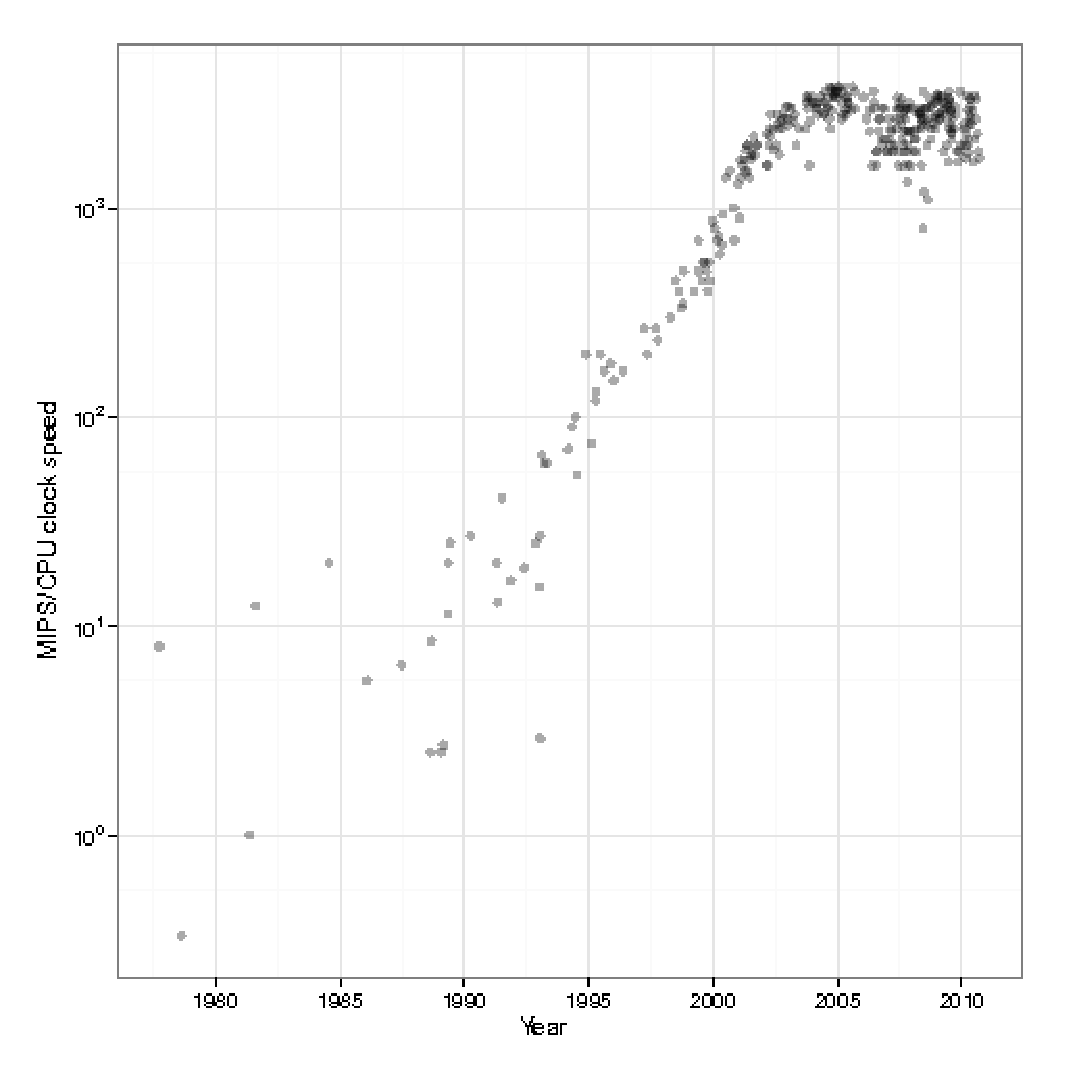
\includegraphics[width=0.5\textwidth]{cpu_and_gpu_trends}
	\caption{Evolutia puterii de procesare\cite{cpu_and_gpu_trends} }
	\label{fig:cpu_and_gpu_trends}
\end{figure}

\begin{figure}
	\centering
	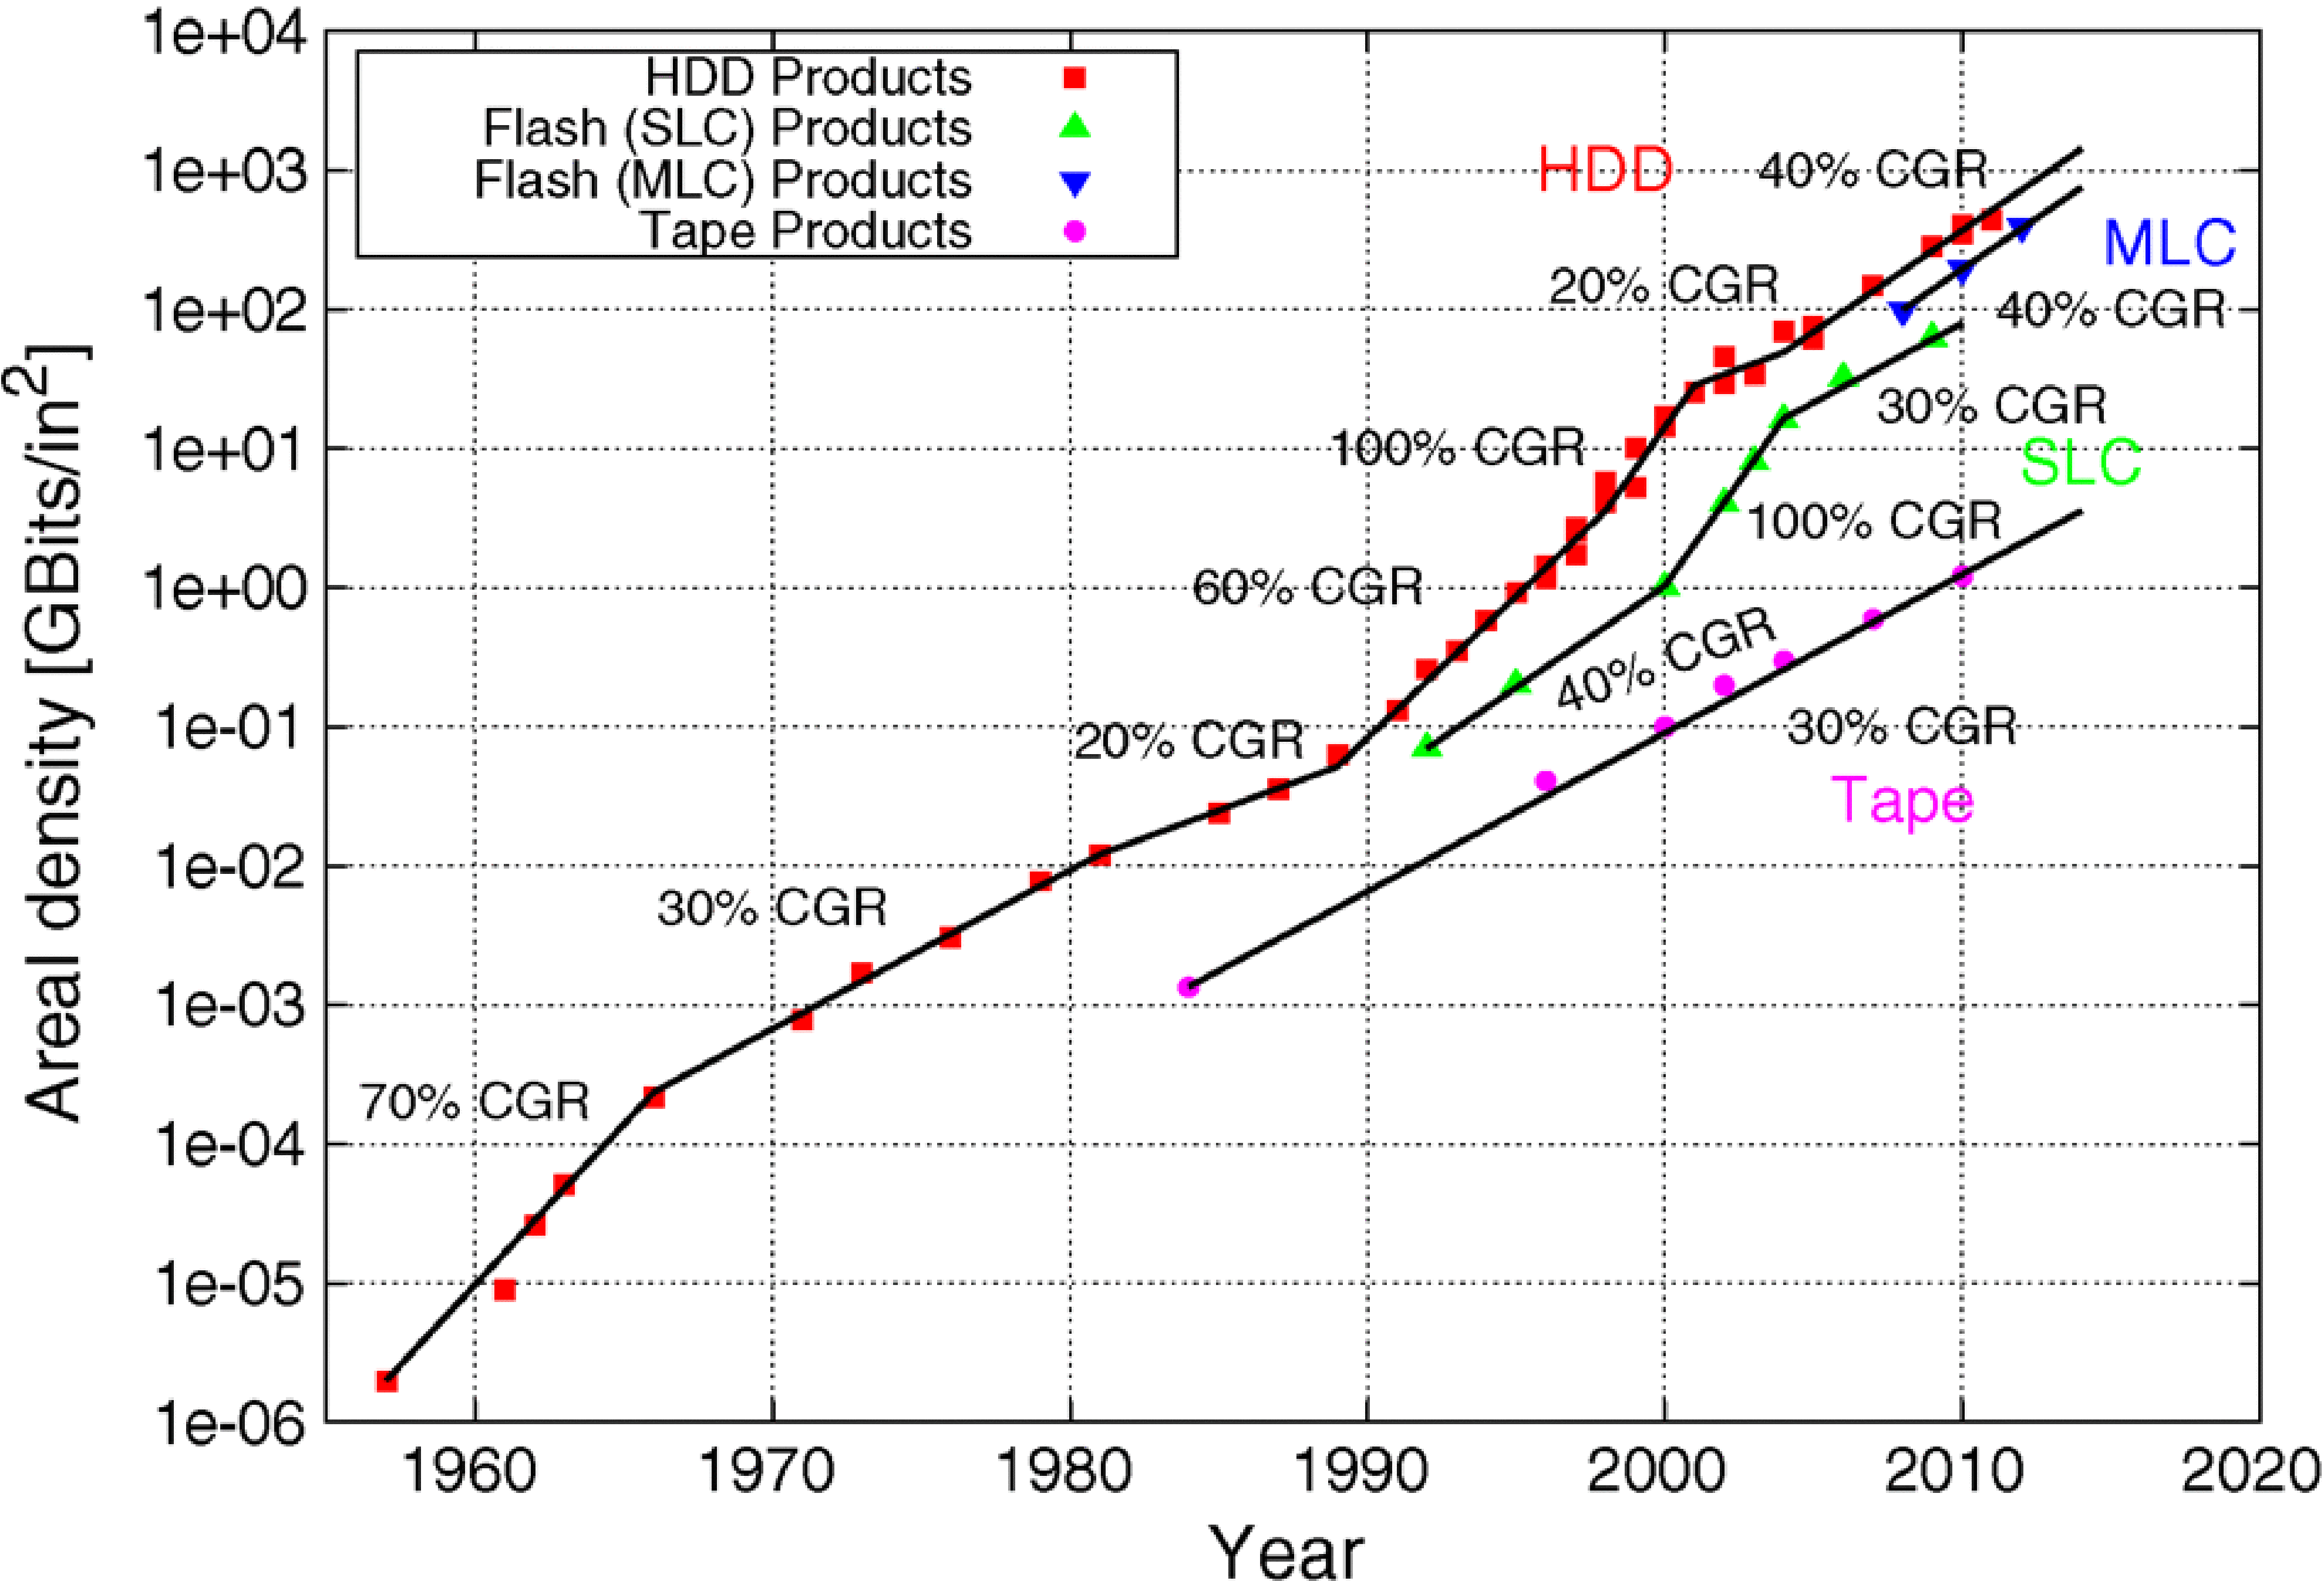
\includegraphics[width=0.5\textwidth]{memory_trends}
	\caption{Evolutia puterii de procesare\cite{memory_trends} }
	\label{fig:memory_trends}
\end{figure}


\chapter{Optimizari de dimensiune}\label{capitolul_optimizari_de_dimensiune}

\section{Eliminarea functiilor nefolosite}

Aceasta lucrare contine o abordare de optimizare a dimensiunii
programelor bazata pe eliminarea functiilor nefolosite.

Desi metrica principala este aceea de dimensiune, reducerea
numarului de instructiuni ale programului poate avea si beneficii
asupra vitezei de executie, din cauza interactiunilor cu cache-ul
calculatoarelor. Pe de alta parte, acest beneficiu este destul de
minor, si nu preprezinta principala motivatie.

In continuare, voi descrie conceptele necesare pentru a intelege
cum putem implementa acest fel de optimizare.

\section{Functie/Metoda}

In domeniul limbajelor de programare, o functie \s{F} este
formata dintr-o colectie de instructiuni tratate ca un întreg,
impreuna cu un protocol pentru executarea acelor instructiuni.

O metoda \s{M} reprezinta o functie asociata unei clase.

In limbajul Java este imposibil sa avem o functie care sa nu
apartina unei metode.
Desi definitiile nu sunt echivalente, deoarece in Java nu exista
functii propriu-zise, ci doar metode, termenii de functie si de metoda
sunt considerati interschimbabili.

Protocolul de executare a functiilor variaza de la limbaj la
limbaj si nu este important pentru scopurile noastre.

De exemplu, functia f
\begin{lstlisting}[language=Python, numbers=left, firstnumber=0]
def f(a, b, c):
    a = a + b
    return c
\end{lstlisting}
contine 2 instructiuni, corespunzatoare liniilor 1-2:

$(i_1)\ a = a + b$

$(i_2)\ return\ c$

Desi in acest exemplu functia \s{F} incepe de pe pozitia 0,
intr-un program format din mai multe functii locul de inceput al
functiei variaza (indicele primei instructiuni).

Vom spune ca doua instructiuni sunt egale daca se afla pe aceeasi
linie. i.e., reprezinta aceeasi pozitie in program.

Pentru programul format din
\begin{lstlisting}[language=Python, numbers=left, firstnumber=0]
def g(a, b, c):
    a = a + b
    a = a * b
    return a
def f(a, b, c):
    a = a + b
    return c
\end{lstlisting}
instructiunile $i_1$ si $i_5$ \textbf{nu} sunt egale.

Vom spune ca o instructiune $\mathbf{i}$ apartine functiei
\s{F} ddaca exista o linie a lui \s{F} unde putem gasi
instructiunea respectiva.

\section{Punctul de intrare principal}

Fie \s{P} un program, executat in ordine secventiala.
Punctul principal de intarare al lui \s{P} reprezinta locul de
unde incepe executia programului -- prima instructiune executata.

Acest loc va fi notat cu \texttt{main}.

\section{Sirul de executie al unui program}

Un sir de executie \s{S} al programului \s{P} reprezinta o inaltuire
finita de instructiuni executate secvential, incepand cu
\texttt{main} si terminandu-se cu ultima instructiune executata de
catre \s{P} inainte ca programul sa se termine.
Pentru ca un sir de executie \s{S} sa fie valid, trebuie sa
existe un input pe care, daca rulam programul, acesta sa
execute fix instructiunile lui \s{S}.

\section{Functii nefolosite}

O functie a unei clase poate fi eliminata daca nu exista niciun
sir de executie valid al programului care sa treaca prin acea
functie.

Vom nota cu $elim(\mathcal{F}) = 1$ daca functia \s{F} poate fi
eliminata deoarece este nefolosita.

Cu alte cuvinte, $elim(\mathcal{F}) = 1$ ddaca

\[
	\text{Pentru oricare } \mathcal{S} \text{ sir de executie, nu
		exista } \mathbf{i} \text{ din } \mathcal{S} \text { care sa faca
		parte din corpul functiei } \mathcal{F}.
\]

\subsection{Sirurile de executie - in practica}

Problema determinarii tuturor sirurilor de executie ale unui
program este o problema grea, intrucat aceasta ar implica rularea
programului pe fiecare input posibil.

Din cauza ca unele programe pot sa fie definite doar partial
(comportamentul lor sa fie nedefinit pe anumite clase de input),
aceasta problema poate fi echivalenta cu Problema Opririi (eng. "The
Halting Problem") \cite{the_halting_problem}: nu avem cum sa stim
daca un input al programului este bun sau nu fara sa rulam
programul, insa nu putem determina daca un program se va termina
vreodata.

Deoarece problema opririi este intractabila, determinarea tuturor
sirurilor de executie posibile ale lui program arbitrar este de
asemenea o problema intractabila.

\subsection{Supersirul de executie}\label{supersirul_de_executie}

Aceasta lucrare va construi o aproximare -- un "supersir" de executie format
dintr-o superpozitie a tuturor sirurilor de executie existente, inclusiv pe cele
invalide (pentru care nu exista un input care sa le genereze).

De exemplu, pentru programul
\begin{lstlisting}[language=Python, numbers=left]
def main():
    if False:
        f()

def f():
    if True:
        return
    g()

def g():
    pass

def h():
    pass
\end{lstlisting}

sirul de executie folosit in problema noastra va contine si
secventa corespunzatoare lantului de apeluri \(main() -> f()\),
cat si lantului \(main() -> f() -> g()\),
chiar daca acestea sunt invalide.

Totodata, sirul de executie generat \textbf{nu} va contine
secventa \(main() -> h()\), sau orice secventa care sa il contina
pe h, din cauza ca aceste secvente nu sunt siruri de executie
(nu exista nicio secventa de instructiuni secventiale
care sa porneasca din functia \texttt{main} si sa ajunga in
functia h).

\subsection{Graful apelurilor de functii}\label{graful_apelurilor}

Vom construi un graf \s{G} al metodelor: fiecarui nod ii va
corespunde o metoda prezenta in program, iar fiecare metoda va
avea un singur nod corespunzator.

Supersirul de executie considera toate secventele de instructiuni
dintr-o metoda, chair daca acestea sunt invalide.
Prin urmare, toate posibilele cai de apel vor fi considerate de
catre acesta.

Asadar, putem reduce problema constructiei supersirului la
problema construirii grafului \s{G}.

In acest graf, exista o muchie de la metoda F la metoda
G daca in secventa de instructiuni a lui F (corpul functiei)
exista un apel catre functia G.

Avand acest graf generat, putem computa multimea \s{M} a metodelor
care sunt accesibile pornind din nodul corespunzator functiei care
contine punctului principal de intrare.
Pentru a optimiza programul, vom elimina toate metodele care nu
apartin acestei multimi.

Demonstratie ca acest procedeu este corect:
\begin{lemma}

	Fie m o metoda care nu apartine lui \s{M}.

	Acest fapt inseamna ca in supersirul de executie nu exista nicio
	instructiune care sa apartina lui m.

	Cum supersirul de executie include toate sirurile de executie
	valide, inseamna ca nu exista niciun sir de executie valid care,
	la un moment dat, sa apeleze functia m.

	Prin urmare, programul obtinut prin eliminarea functiei m va fi
	echivalent cu programul initial.
\end{lemma}

\subsection{Algoritmul pentru eliminarea
functiilor}\label{algoritm_naiv_pentru_eliminare}

Pentru a construi graful, trebuie sa putem deduce pentru fiecare
metoda care sunt metodele pe care aceasta le apeleaza.
Acest lucru este dependent de limbajul asupra caruia se aplica
optimizarea, asadar il vom considera deja implementat.

Putem considera astfel functia
\begin{lstlisting}[language=Python]
def direct_calees(m: Method) -> [Method]
    return all methods directly called by m.
\end{lstlisting}
ca fiind la dispozitia noastra.

Pentru a forma multimea metodelor accesibile din \texttt{main},
putem utiliza o parcugere in latime a grafului.

\begin{lstlisting}[language=Python]
def reachable_methods(main: Method) -> [Method]:
    coada = [main]
    at = 0
    while at < size(coada):
        m = coada[at]
        at = at + 1
        for next in direct_calees(m):
            if next not in coada:
                coada.push(next)
    return coada
\end{lstlisting}

Avand multimea generata, ramane doar sa eliminam functiile
care nu fac partea din ea:

\begin{lstlisting}[language=Python]
def optimize_for_size(p: Program) -> Program:
    main = p.main_method()
    used_methods = reachable_methods(main)
    for m in p.all_methods():
        if m not in used_methods:
            p.remove_method(m)
    return p
\end{lstlisting}

\chapter{Detaliile tehnice ale limbajului Java}

În acest capitol vom detalia limbajul Java și modul de
funcționare a acestuia.

\section{Limbajul Java}

Java este un limbaj de programare orientat pe obiecte. Acesta a fost
dezvoltat de către Sun Microsystems (acum Oracle), iar prima versiune a
apărut în anul 1995.

Java s-a bazat pe sintaxa limbajului C, și a introdus noțiunea de
``scrie o data, rulează peste tot'' (Eng. ``write once, run
everywhere''). Spre deosebire de C și de C++, care trebuiesc compilate
pentru fiecare platformă țintă, Java a avut avantajul că trebuie
compilat o singura data, și va merge garantat pe toate platformele
suportate de limbaj.

\section{Java Bytecode}

Soluția limbajului Java pentru a fi independent de platformă este de a
transforma codul într-o reprezentare intermediara, în loc de direct în
cod binar pentru o anumită arhitectură .

Compilatorul Java (\texttt{javac}), transformă codul Java într-un limbaj
intermediar, numit Java Bytecode.

Acest limbaj este un limbaj de nivel scăzut (Eng. "low-level"), destinat în mod exclusiv
procesării de către mașini, spre deosebire de codul Java, care este
destinat oamenilor.

După ce compilatorul a procesat codul Java, provenit din fișiere .java în
format text, acesta salvează rezultatul în fișiere de tip clasă (.class)
în format binar.

\section{JVM}

Odată generate fișierele binare, acestea sunt executate pe o mașina
virtuală specifica limbajului Java --- numită \texttt{JVM}
(Eng. Java Virtual Machine).

Această mașina virtuală are rolul de a citi fișierele de clasă binare și
de a le interpreta.

Mașina virtuală este implementată ca o ``mașină cu stivă'' (Eng. Stack
machine), unde toate instrucțiunile limbajului bytecode interacționează
cu datele de pe o stivă controlată de aplicație.

Mașina virtuală însuși este implementată în C/C++, și este compilată în
cod binar direct, dependent de arhitectura calculatorului. Dezvoltatorii limbajului
Java sunt responsabili pentru corectitudinea și siguranța mașinii
virtuale, în timp ce dezvoltatorii de aplicații Java au garanția că dacă
codul lor Java este corect, atunci acesta va rula la fel, deterministic,
pe orice platforma.

În acestă privință, limbajul Java poate fi văzut ca un limbaj interpretat.
Comparând cu alte limbaje populare interpretate, ca de exemplu Python,
Ruby, sau Perl, ne-am aștepta ca și Java să fie la fel de încet ca
acestea~\cite{language_benchmarks}.
Totuși, Java obține performanțe mult mai bune decât
acestea. Acest fapt se datorează compilării tocmai-la-timp (Eng.\
just-in-time), în care atunci când interpretorul observă o secventa de
cod care este interpretată repetitiv de foarte multe ori, va genera
direct cod binari pentru aceasta.


\section{Fișierele clasa}

Fișierele de clasa Java sunt formate din 10
secțiuni~\cite{classfile_sections}:

\begin{enumerate}
	\item
	      Constanta magică.
	\item
	      Versiunea fișierului.
	\item
	      Constantele clasei.
	\item
	      Permisiunile de acces.
	\item
	      Numele clasei din fișier.
	\item
	      Numele super clasei.
	\item
	      Interfețele pe care clasa le implementează.
	\item
	      Câmpurile clasei.
	\item
	      Metodele clasei.
	\item
	      Atribute ale clasei.
\end{enumerate}

În continuare voi da o scurta descriere a formatului secțiunilor.

\section{Secțiunile fișierelor clasa}

\subsection{Magic}

Toate fișierele clasă trebuiesc să înceapă cu un număr denumit constanta
magică. Acesta este folosit pentru a identifica în mod unic că acestea
sunt într-adevăr fișiere clasă. Numărul magic are o valoare memorabilă:
reprezentarea hexadecimală este \texttt{0xCAFEBABE},

\subsection{Versiunea}

Versiunea unui fișier clasă este dată de doua valori, versiunea majoră
\texttt{M} și versiunea minoră \texttt{m}. Versiunea clasei este atunci
reprezentata ca \texttt{M.m}. (e.g., \texttt{45.1}). Aceasta este
folosită pentru a menține compatibilitatea în cazul modificărilor
mașinii virtuale care interpretează clasa sau ale compilatorului care o
generează.

\subsection{Constantele clasei}

Tabela de constante este locul unde sunt stocate valorile literale
constante ale clasei:

\begin{itemize}
	\item Numere întregi.
	\item Numere cu virgula mobilă.
	\item Șiruri de caractere, care pot reprezenta la rândul lor:
	      \begin{itemize}
		      \item Nume de clase.
		      \item Nume de metode.
		      \item Tipuri ale metodelor.
	      \end{itemize}
	\item Informații compuse din datele anterioare:
	      \begin{itemize}
		      \item Referința către o metodă a unei clase.
		      \item Referința către o constantă a unei clase.
	      \end{itemize}
\end{itemize}

Toate celelalte tipuri de date compuse, cum ar fi metodele sau
câmpurile, vor conține indecși în tabela de constante.

Aproape toate tipurile de constante ocupă o singură poziție în tabelă, însă, din
motive istorice, unele constante ocupă două poziții.
Tot din motive istorice, tabela este indexată de la 1, și nu
de la 0, cum sunt celelalte.

\subsection{Permisiunile de acces}

Aceste permisiuni constau într-o mască de biți, care reprezintă
operațiile permise pe această clasă:

\begin{itemize}
	\item dacă clasa este publică, și poate fi accesată din afara pachetului acesteia.
	\item dacă clasa este finala, și dacă poate fi extinsă.
	\item dacă invocarea metodelor din super clasă să fie tratata special.
	\item dacă este de fapt o interfață, și nu o clasă.
	\item dacă este o clasă abstractă și nu poate fi instanțiată.
\end{itemize}

\subsection{Clasa curentă}

Reprezintă un indice în tabela de constante, unde sunt stocate
informații despre clasa curentă.

\subsection{Clasa super}

Reprezintă un indice în tabela de constante, cu informații despre clasa
din care a moștenit clasa curentă. Dacă este 0, clasa
curentă nu moștenește nimic: singura clasă fără o super clasă este
Object.

E.g. Pentru

\begin{lstlisting}[language=Java]
public class MyClass extends S implements I
\end{lstlisting}

Indicele corespunde lui \texttt{S}.

\subsection{Interfețele}

Reprezintă o colecție de indici în tabela de constante. Fiecare valoare
de la acei indici constituie o interfață implementată în mod direct de
către clasa curentă. Interfețele apar în ordinea declarată în fișierele
Java.

E.g. Pentru

\begin{lstlisting}[language=Java]
class MyClass extends S implements I1, I2
\end{lstlisting}

Primul indice ar corespunde lui \texttt{I1}, iar al doilea lui
\texttt{I2}.

\subsection{Câmpurile}\label{campurile}

Reprezintă informații despre câmpurile (Eng. Fields) clasei:
\begin{itemize}
	\item Permisiunile de acces: dacă este public sau privat, etc.
	\item Numele câmpului.
	\item Tipul câmpului.
	\item Alte atribute: dacă este depreciat, dacă are o valoare constantă, etc.
\end{itemize}

\subsection{Metodele}\label{metodele}

Reprezintă informații despre toate metodele clasei, inclusiv
constructorii:

\begin{itemize}
	\item Permisiuni de acces: dacă este publică sau privată,
        dacă este finală , dacă este abstractă.
	\item Numele metodei.
	\item Tipul metodei.
	\item În caz că nu este abstractă, codul metodei.
	\item Alte atribute:
	      \begin{itemize}
		      \item Ce excepții poate arunca.
		      \item Dacă este depreciată.
	      \end{itemize}
\end{itemize}

Codul metodei este partea cea mai importantă, iar formatul acestuia
urmează să fie detaliat ulterior.

\subsection{Atributele}

Reprezintă alte informații despre clasă, cum ar fi:
\begin{itemize}
	\item Clasele definite în interiorul acesteia.
	\item În caz că este o clasă anonimă sau definită local, metoda în care este definită.
	\item Numele fișierul sursă din care a fost compilată clasa.
\end{itemize}

\section{Tipuri de date}

În continuare, voi descrie din punct de vedere tehnic tipurile de date
întâlnite în fișierele de clasă.

\subsection{Tipuri de baza}

În formatul fișierelor clasa există trei tipuri elementare, toate bazate pe
întregi. În caz că un întreg are mai mulți octeți, aceștia au ordinea de
\texttt{big-endian}: cel mai semnificativ octet va fi mereu primul în
memorie.

\begin{longtable}[]{@{}ccc@{}}
	\toprule
	Nume        & Semantica                       & Echivalentul în C\tabularnewline
	\midrule
	\endhead
	\texttt{u1} & întreg pe un octet, fără semn   & \texttt{unsigned\ char}
	sau \texttt{uint8\_t}\tabularnewline
	\texttt{u2} & întreg pe doi octeți, fără semn & \texttt{unsigned\ short}
	sau \texttt{uint16\_t}\tabularnewline
	\texttt{u4} & întreg pe un octet, fără semn   & \texttt{unsigned\ int} sau
	\texttt{uint32\_t}\tabularnewline
	\bottomrule
\end{longtable}

În codul sursă al proiectului, acestea sunt tratate astfel:

\begin{lstlisting}[language=C++]
using u1 = uint8_t;
using u2 = uint16_t;
using u4 = uint32_t;
\end{lstlisting}

\subsection{Tipuri compuse}

\subsection{Constantele}

Fiecare constantă din tabela de constante începe cu o etichetă de 1
octet, care reprezintă datele și tipul structurii. Conținutul acesteia
variază în funcție de etichetă, însa indiferent de etichetă, conținutul
trebuie să aibă cel puțin 2 octeți.

\subsubsection{CONSTANT\_Class}

Corespunde valorii etichetei de 7 și conține un indice spre un alt câmp
în tabela de constante, de tipul \texttt{CONSTANT\_Utf8} --- un șir de
caractere. Acel șir de caractere va conține numele clasei.

\subsubsection{CONSTANT\_Fieldref}

Corespunde valorii etichetei de 9 și conține o referință spre câmpul
unei clase. Referința constă în doi indici, amândoi care arată spre
tabela de constante. Primul indice arată spre o constantă
\texttt{CONSTANT\_Class}, care reprezintă clasa sau interfața căreia
aparține metoda. Al doilea indice arată spre o constantă
\texttt{CONSTANT\_NameAndType}, care conține informații despre numele și
tipul câmpului.

\subsubsection{CONSTANT\_Methodref}

Corespunde valorii etichetei de 10 și conține o referința spre metoda
unei clase. Are o structură identică cu \texttt{CONSTANT\_Fieldref},
doar că primul indice arată neapărat spre o clasă, în timp ce al doilea
indice arată spre numele și tipul metodei.

\subsubsection{CONSTANT\_InterfaceMethodref}

Corespunde valorii etichetei de 11 și conține o referință spre metoda
unei interfețe. Are o structura identică cu
\texttt{CONSTANT\_Methodref}, doar că primul indice arată spre o
interfață.

\subsubsection{CONSTANT\_String}

Corespunde valorii etichetei de 8 și reprezintă un șir de caractere.
Conține un indice către o structură de tipul \texttt{CONSTANT\_Utf8}.

\subsubsection{CONSTANT\_Integer}

Corespunde valorii etichetei de 3 și conține un întreg pe 4 octeți.

\subsubsection{CONSTANT\_Float}

Corespunde valorii etichetei de 4 și conține un număr cu virgulă mobilă
pe 4 octeți.

\subsubsection{CONSTANT\_Long}

Corespunde valorii etichetei de 5 și conține un întreg pe 8 octeți. Din
motive istorice, ocupă 2 spatii în tabela de constante.

\subsubsection{CONSTANT\_Double}

Corespunde valorii etichetei de 6 și conține un număr cu virgulă mobilă
pe 8 octeți. Din motive istorice, ocupă 2 spatii în tabela de constante.

\subsubsection{CONSTANT\_NameAndType}

Corespunde valorii etichetei de 12. Descrie numele și tipul unui câmp
sau al unei metode, fără informații despre clasă. Conține doi indici,
amândoi către structuri de tipul \texttt{CONSTANT\_Utf8}. Primul
reprezintă numele, iar al doilea tipul.

\subsubsection{CONSTANT\_Utf8}

Corespunde valorii etichetei de 1. Reprezintă un șir de caractere
encodat în formatul UTF-8. Conține un întreg \texttt{length}, de tipul
\texttt{u2}, și apoi \texttt{length} octeți care descriu șirul în sine.
Din cauza că este encodat ca UTF-8, un singur caracter poate fi format
din mai multi octeți.

\subsubsection{CONSTANT\_MethodHandle}

Corespunde valorii etichetei de 15 și conține o referințe către un câmp,
o metodă de clasă, sau o metodă de interfață.

\subsubsection{CONSTANT\_MethodType}

Corespunde valorii etichetei de 16 și conține un indice către o
constantă \texttt{CONSTANT\_Utf8}, ce reprezintă tipul unei metode.

\subsubsection{CONSTANT\_InvokeDynamic}

Corespunde valorii etichetei de 18 și este folosit de către \texttt{JVM}
pentru a invoca o metodă polimorfică.

În cod \texttt{C++}, am reprezentat \texttt{cp\_info} astfel:

\begin{lstlisting}[language=C++]
struct cp_info {
    enum class Tag : u1 {
        CONSTANT_Class = 7,
        CONSTANT_Fieldref = 9,
        CONSTANT_Methodref = 10,
        CONSTANT_InterfaceMethodref = 11,
        CONSTANT_String = 8,
        CONSTANT_Integer = 3,
        CONSTANT_Float = 4,
        CONSTANT_Long = 5,
        CONSTANT_Double = 6,
        CONSTANT_NameAndType = 12,
        CONSTANT_Utf8_info = 1,
        CONSTANT_MethodHandle = 15,
        CONSTANT_MethodType = 16,
        CONSTANT_InvokeDynamic = 18,
    };

    Tag tag;
    std::vector<u1> data;
};
\end{lstlisting}

Iar structurile folosite pentru obiectivul propus au fost reprezentate
astfel~\cite{classfile_sections}:

\begin{lstlisting}[language=C++]
struct CONSTANT_Methodref_info {
    cp_info::Tag tag;
    u2 class_index;
    u2 name_and_type_index;
};
struct CONSTANT_Class_info {
    cp_info::Tag tag;
    u2 name_index;
};
struct CONSTANT_NameAndType_info {
    cp_info::Tag tag;
    u2 name_index;
    u2 descriptor_index;
};
\end{lstlisting}

\paragraph{\texorpdfstring{\texttt{field\_info}}{field\_info}}\label{field_info}

Fiecare câmp din cadrul unei clase este reprezentat printr-o structură
de tipul \texttt{field\_info}.

În cod \texttt{C++}, această structură a fost reprezentată astfel~\cite{classfile_sections}:

\begin{lstlisting}[language=C++]
struct field_info {
    u2 access_flags;
    u2 name_index;
    u2 descriptor_index;
    u2 attributes_count;
    std::vector<attribute_info> attributes;
};
\end{lstlisting}

Unde:
\begin{itemize}
	\item \texttt{name\_index} este o intrare în tabela de constante unde se afla o constantă de tipul \texttt{CONSTANT\_Utf8}.
	\item \texttt{descriptor\_index} arată spre o constantă de tipul \texttt{CONSTANT\_Utf8} și reprezintă tipul câmpului.
\end{itemize}

\paragraph{\texorpdfstring{\texttt{method\_info}}{method\_info}}\label{method_info}

Fiecare metodă a unei clase/interfețe este descrisă prin această
structură.

În cod \texttt{C++}, am implementat-o astfel~\cite{classfile_sections}:

\begin{lstlisting}[language=C++]
struct method_info {
    u2 access_flags;
    u2 name_index;
    u2 descriptor_index;
    u2 attributes_count;
    std::vector<attribute_info> attributes;
};
\end{lstlisting}

Unde \texttt{name\_index} și \texttt{descriptor\_index} au aceeași
interpretare ca și la \texttt{field\_info}.

Dacă metoda nu este abstractă, atunci în vectorul \texttt{attributes} se
va găsi un atribut de tipul \texttt{Code}, care conține bytecode-ul
corespunzător acestei metode.

\paragraph{\texorpdfstring{\texttt{attribute\_info}}{attribute\_info}}\label{attribute_info}

În \texttt{C++}, a fost implementată astfel~\cite{classfile_sections}:

\begin{lstlisting}[language=C++]
struct attribute_info {
    u2 attribute_name_index;
    u4 attribute_length;
    std::vector<u1> info;
};
\end{lstlisting}

Numele atributului determină modul în care octeții din vectorul
\texttt{info} sunt interpretați.

\subsubsection{Atributul de cod}

Pentru intențiile noastre, atributul de interes este cel de cod~\cite{classfile_sections}:

\subparagraph{\texorpdfstring{\texttt{Code\_attribute}}{Code\_attribute}}\label{code_attribute}

\begin{lstlisting}[language=C++]
struct Code_attribute {
    u2 attribute_name_index;
    u4 attribute_length;

    u2 max_stack;
    u2 max_locals;

    u4 code_length;
    std::vector<u1> code;

    u2 exception_table_length;
    struct exception {
        u2 start_pc;
        u2 end_pc;
        u2 handler_pc;
        u2 catch_type;
    };
    std::vector<exception> exception_table; // of length exception_table_length.
    u2 attributes_count;
    std::vector<attribute_info> attributes; // of length attributes_count.
};
\end{lstlisting}

Această structură este esențială pentru implementarea optimizării,
întrucât ea ne permite să determinăm metodele apelate din cadrul unei secvente de cod.
În continuare, o voi descrie detaliat:

\begin{itemize}
	\tightlist
	\item
	      \texttt{max\_stack}: Reprezintă adâncimea maximă a stivei mașinii
	      virtuale când această bucată de cod este interpretată.
	\item
	      \texttt{max\_locals}: Reprezintă numărul maxim de variabile locale
	      alocate în același timp când această bucată de cod este interpretată.
	\item
	      \texttt{code}: Codul metodei.
	\item
	      \texttt{exception\_table}: Excepțiile pe care le poate arunca metoda.
\end{itemize}

\subsubsection{Code}

Vectorul \texttt{code} din cadrul atributului \texttt{Code} reprezintă
bytecode-ul propriu-zis al metodei.

Acest vector conține instrucțiunile care sunt executate de către mașina
virtuală.

JVM-ul rulează ca o mașina cu stivă, iar toate instrucțiunile operează
pe această stivă. Rezultatul rulării unei instrucțiuni este modificarea
stivei: scoaterea și adăugarea de elemente în vraful acesteia.

Instrucțiunile au în general formatul~\cite{instruction_format}

\begin{verbatim}
nume_instr
operand1
operand2
...
\end{verbatim}

Cu un număr variabil de operanzi, prezenți în mod explicit în vectorul
de \texttt{cod}.

Fiecărei instrucțiuni îi corespunde un octet, denumit opcode. Fiecare
operand este fie cunoscut la compilare, fie calculat în mod dinamic la
rulare.

Cele mai multe operații nu au niciun operand dat în mod explicit la
nivelul instrucțiunii --- ele lucrează doar cu valorile din vârful stivei
la momentul execuției codului.

De exemplu:

Instrucțiunea \texttt{imul} are octetul 104 sau 0x68.
Aceasta extrage două valori din vârful stivei: \texttt{value1} și
\texttt{value2}. Ambele valori trebuie să fie de tipul \texttt{int}.
Rezultatul este înmulțirea celor două valori:
\texttt{result\ =\ value1\ *\ value2}, și este pus în vârful stivei.

Dintre cele peste o sută de instrucțiuni, noi suntem preocupați doar de
5 dintre acestea: cele care au de a face cu invocarea unei metode.

\textbf{invokedynamic}

Format:
\begin{verbatim}
invokedynamic
index1
index2
0
0
\end{verbatim}

Opcode-ul corespunzător acestei instrucțiuni este 186 sau
0xba~\cite{instruction_format}.

Index1 și index2 sunt doi octeți. Aceștia sunt compuși în
\begin{lstlisting}
index = (index1 << 8) | index2
\end{lstlisting}
Unde \texttt{<<} reprezintă shiftare pe biți, iar \texttt{|}
reprezintă operația de sau pe biți.

Indicele compus reprezintă o intrare în tabela de constante. La locația
respectivă trebuie să se afle o structură de tipul
\texttt{CONSTANT\_MethodHandle}

\textbf{invokeinterface}

Format:
\begin{verbatim}
invokeinterface
index1
index2
count
0
\end{verbatim}

Opcode-ul corespunzător este 185 sau 0xb9~\cite{instruction_format}.
\texttt{index1} și \texttt{index2} sunt folosiți, în mod similar ca la
\texttt{invokedynamic}, pentru a construi un indice în tabela
de constante.

La poziția respectivă în tabelă, trebuie să se găsească o structură de
tipul \texttt{CONSTANT\_Methodref}.

\texttt{count} trebuie să fie un octet fără semn diferit de 0. Acest
operand descrie numărul argumentelor metodei, și este necesar din motive
istorice (aceasta informație poate fi dedusa din tipul metodei).

\textbf{invokespecial}

Format:
\begin{verbatim}
invokespecial
index1
index2
\end{verbatim}

Opcode-ul corespunzător este 183 sau 0xb7~\cite{instruction_format}. La fel ca la
\texttt{invokeinterface}, instrucțiunea conține un indice în tabela de constante
către o structură \texttt{CONSTANT\_Methodref}.

Această instrucțiune este folosită pentru a invoca constructorii
claselor.

\textbf{invokestatic}

Format:
\begin{verbatim}
invokestatic
index1
index1
\end{verbatim}

Opcode-ul corespunzător este 184 sau 0xb8~\cite{instruction_format}.
Instrucțiunea invocă o metodă statică a unei clase.

La fel ca la \texttt{invokeinterface}, este construit un indice compus,
și folosit pentru a indexa tabela de constante.

\textbf{invokevirtual}

Format:
\begin{verbatim}
invokevirtual
index1
index1
\end{verbatim}

Opcode-ul corespunzător este 182 sau 0xb6~\cite{instruction_format}, iar
interpretarea este la fel ca la \texttt{invokeinterface}.
Aceasta este cea mai comună
instrucțiune de invocare de funcții.

În \texttt{C++}, am reprezentat aceste instrucțiuni de interes astfel:

\begin{lstlisting}[language=C++]
enum class Instr {
    invokedynamic = 0xba,
    invokeinterface = 0xb9,
    invokespecial = 0xb7,
    invokestatic = 0xb8,
    invokevirtual = 0xb6,
};
\end{lstlisting}

\subsection{ClassFile}\label{classfile}

Folosind definițiile anterioare, putem descrie un fișier de clasă binar
în C++:

\begin{lstlisting}[language=C++]
struct ClassFile {
    u4 magic; // Should be 0xCAFEBABE.

    u2 minor_version;
    u2 major_version;

    u2 constant_pool_count;
    std::vector<cp_info> constant_pool;

    u2 access_flags;

    u2 this_class;
    u2 super_class;

    u2 interface_count;
    std::vector<interface_info> interfaces;

    u2 field_count;
    std::vector<field_info> fields;

    u2 method_count;
    std::vector<method_info> methods;

    u2 attribute_count;
    std::vector<attribute_info> attributes;
};
\end{lstlisting}

Pentru a vedea un fișier clasa analizat în detaliu, va puteți
uita la appendix-ul Studiu de Caz \ref{appendix:studiu_de_caz}.

\chapter{Limbajul Java si optimizarea acestuia}

In prima parte, vom detalia limbajul Java si modul de functionare
a acestuia.
In a doua parte, vom descrie cum putem implementa optimizarea
eliminarii de metode nefolosite in limbajul Java.

\section{Limbajul Java}

Java este un limbaj de programare orientat pe obiecte. Acesta a fost
dezvoltat de catre Sun Microsystems (acum Oracle), iar prima versiune a
aparut in anul 1995.

Jaza s-a bazat pe sintaxa limbajului C, si a introdus notiunea de
``scrie o data, ruleaza peste tot'' (eng. ``write once, run
everywhere''). Spre deosebire de C si de C++, care trebuiesc compilate
pentru fiecare platforma tinta, Java a avut avantajul ca trebuie
compilat o singura data, si va merge garantat pe toate platformele
suportate de limbaj.

\section{Java Bytecode}

Solutia limbajului Java pentru a fi independent de platforma este de
transforma codul intr-o reprezentare intermediara, in loc de direct in
cod binary pentru o anumita arhitectura .

Compilatorul Java (\texttt{javac}), transforma codul Java intr-un limbaj
intermediar, numit Java Bytecode.

Acest limbaj este un limbaj low-level, destinat in mod exclusiv
procesarii de catre masini, spre deosebire de codul Java, care este
destinat oamenilor.

Dupa ce compilatorul a procesat codul Java, provenit din fisere .java in
format text, acesta salveaza rezultatul in fisiere de tip clasa (.class)
in format binar.

\section{JVM}

Odata generate fisierele binare, acestea sunt executate pe o masina
virtuala specifica limbajului Java --- numita \texttt{JVM}
(eng. Java Virtual Machine).

Aceasta masina virtuala are rolul de a citi fisierele de clasa binare si
de a le interpreta.

Masina virtuala este implementata ca o ``masina cu stiva'' (eng. stack
machine), unde toate instructiunile limbajului bytecode interactioneaza
cu datele de pe o stiva controlata de aplicatie.

Masina virtuala insusi este implementata in C/C++, si este compilata in
cod binar direct, dependent de arhitectura. Dezvoltatorii limbajului
Java sunt responsabili pentru corectitudinea si siguranta masinii
virtuale, in timp ce dezvoltatorii de aplicatii Java au garantia ca daca
codul lor Java este corect, atunci acesta va rula la fel, deterministic,
pe orice platforma.

In acest regard, limbajul Java poate fi vazut ca un limbaj interpretat.
Comparand cu alte limbaje populare interpretate, ca de exemplu Python,
Ruby, sau Perl, ne-am astepta ca si Java sa fie la fel de incet ca
acestea~\cite{language_benchmarks}.
Totusi, Java obtine performante mult mai bune decat
aceastea. Acest fapt se datoreaza compilarii tocmai-la-timp (eng.\
just-in-time), in care atunci cand interpretorul observa o secventa de
cod care este interpretata repetitiv de foarte multe ori, va genera
direct cod binary pentru aceasta.

\section{Fisierele clasa}

Fisierele de clasa Java sunt formate din 10
sectiuni\cite{classfile_sections}:

\begin{enumerate}
	\item
	      Constanta magica.
	\item
	      Versiunea fisierului.
	\item
	      Constantele clasei.
	\item
	      Permisiunile de acces.
	\item
	      Numele clasei din fisier.
	\item
	      Numele superclasei.
	\item
	      Interfetele pe care clasa le implementeaza.
	\item
	      Campurile clasei.
	\item
	      Metodele clasei.
	\item
	      Atribute ale clasei.
\end{enumerate}

In continuare voi da o scurta descriere a formatului sectiunilor.

\section{Sectiunile fiserelor clasa}

\subsection{Magic}

Toate fiserele clasa trebuiesc sa inceapa cu un numar denumit constanta
magica. Acesta este folosit pentru a identifica in mod unic ca acestea
sunt intra-devar fisiere clasa. Numarul magic are o valoare memorabila:
reprezentarea hexadecimala este \texttt{0xCAFEBABE},

\subsection{Versiunea}

Versiunea unui fisier clasa este data de doua valori, versiunea majora
\texttt{M} si versiunea minora \texttt{m}. Versiunea clasei este atunci
reprezentata ca \texttt{M.m}. (e.g., \texttt{45.1}). Aceasta este
folosita pentru a mentine compatibilitatea in cazul modificarilor
masinii virtuale care interpreteaza clasa sau ale compilatorului care o
genereaza.

\subsection{Constantele clasei}

Tabela de constante este locul unde sunt stocate valorile literale
constante ale clasei:

\begin{itemize}
	\item Numere intregi.
	\item Numere cu virgula mobula.
	\item Siruri de caractere, care pot reprezenta la randul lor:
	      \begin{itemize}
		      \item Nume de clase.
		      \item Nume de metode.
		      \item Tipuri ale metodelor.
	      \end{itemize}
	\item Informatii compuse din datele anterioare:
	      \begin{itemize}
		      \item Referinta la o metoda a unei clase.
		      \item Referinta la o constanta a unei clase.
	      \end{itemize}
\end{itemize}

Toate celelalte tipuri de date compuse, cum ar fi metodele sau
campurile, vor contine indecsi in tabela de constante.

Aproape toate tipurile de constante ocupa un singur slot in tabela, insa, din
motive istorice, unele constante ocupa doua sloturi.
Tot din motive istorice, tabela este indexata de la 1, si nu
de la 0, cum sunt celelalte.

\subsection{Permisiunile de acces}

Aceste permisiuni constau intr-o masca de bitsi, care reprezeinta
operatiile permise pe aceasta clasa:

\begin{itemize}
	\item daca clasa este publica, si poate fi accesta din afara pachetului acesteia.
	\item daca clasa este finala, si daca poate fi extinsa.
	\item daca invocarea metodelor din superclasa sa fie tratata special.
	\item daca este de fapt o interfata, si nu o clasa.
	\item daca este o clasa abstracta si nu poate fi instatiata.
\end{itemize}

\subsection{Clasa curenta}

Reprezinta un indice in tabela de constante, unde sunt stocate
informatii despre clasa curenta.

\subsection{Clasa super}

Reprezinta un indice in tabela de consatante, cu informatii despre clasa
din care a mostenit clasa curenta. Daca este 0, inseamna ca clasa
curenta nu mosteneste nimic: singura clasa fara o superclasa este clasa
Object.

E.g. pentru

\begin{lstlisting}[language=Java]
public class MyClass extends S implements I
\end{lstlisting}

Indicele corespunde lui \texttt{S}.

\subsection{Interfetele}

Reprezinta o colectie de indici in tabela de constante. Fiecare valoare
de la acei indici reprezinta o interfata implementata in mod direct de
catre clasa curenta. Interfetele apar in ordinea declarata in fisierele
java.

E.g. pentru

\begin{lstlisting}[language=Java]
class MyClass extends S implements I1, I2
\end{lstlisting}

Primul indice ar corespunde lui \texttt{I1}, iar al doilea lui
\texttt{I2}.

\subsection{Campurile}\label{campurile}

Reprezinta informatii despre campurile (eng. fields) clasei:
\begin{itemize}
	\item Permisiunile de acces: daca este public sau privat, etc.
	\item Numele campului.
	\item Tipul campului.
	\item Alte atribute: daca este deprecat, daca are o valoare constanta, etc.
\end{itemize}

\subsection{Metodele}\label{metodele}

Reprezinta informatii despre toate metodele clasei, inclusiv
constructorii:

\begin{itemize}
	\item Permisiuni de acces: daca este public sau privat, daca este finala, daca este abstracta.
	\item Numele metodei.
	\item Tipul metodei.
	\item In caz ca nu este abstracta, byte codul metodei.
	\item Alte atribute:
	      \begin{itemize}
		      \item Ce exceptii poate arunca.
		      \item Daca este deprecata.
	      \end{itemize}
\end{itemize}

Codul metodei este partea cea mai importanta, iar formatul acestuia
urmeaza sa fie detaliat ulterior.

\subsection{Atributele}

Reprezinta alte informatii despre clasa, cum ar fi:
\begin{itemize}
	\item Clasele definite in interiorul acesteia.
	\item In caz ca este o clasa anonima sau definita local, metoda in care este definita.
	\item Numele fisierul sursa din care a fost compilata clasa.
\end{itemize}

\section{Tipuri de date}

In continuare, voi descrie din punct de vedere tehnic tipurile de date
intalnite in fisierele de clasa.

\subsection{Tipuri de baza}

In formatul fisierelor clasa exista trei tipuri de baza, toate bazate pe
intregi. In caz ca un intreg are mai multi octeti, acestia au ordinea de
\texttt{big-endian}: cel mai semnificativ octet va fi mereu primul in
memorie.

\begin{longtable}[]{@{}ccc@{}}
	\toprule
	Nume        & Semantica                       & Echivalentul in C\tabularnewline
	\midrule
	\endhead
	\texttt{u1} & intreg pe un octet, fara semn   & \texttt{unsigned\ char}
	sau \texttt{uint8\_t}\tabularnewline
	\texttt{u2} & intreg pe doi octeti, fara semn & \texttt{unsigned\ short}
	sau \texttt{uint16\_t}\tabularnewline
	\texttt{u4} & intreg pe un octet, fara semn   & \texttt{unsigned\ int} sau
	\texttt{uint32\_t}\tabularnewline
	\bottomrule
\end{longtable}

In codul sursa al proiectului, acestea sunt tratate astfel:

\begin{lstlisting}[language=C++]
using u1 = uint8_t;
using u2 = uint16_t;
using u4 = uint32_t;
\end{lstlisting}

\subsection{Tipuri compuse}

\subsection{Tipurile de constante}

Fiecare constanta din tabela de constante incepe cu o eticheta de 1
octet, care reprezinta datele si tipul structurii. Continutul acesteia
variaza in functie de eticheta, insa indiferent de eticheta, continutul
trebuie sa aiba cel putin 2 octeti.

\subsubsection{CONSTANT\_Class}

Corespunde valorii etichetei de 7 si contine un indice spre un alt camp
in tabela de constante, de tipul \texttt{CONSTANT\_Utf8} --- un sir de
caractere. Acel sir de caractere va contine numele clasei.

\subsubsection{CONSTANT\_Fieldref}

Corespunde valorii etichetei de 9 si contine o referinta spre campul
unei clase. Referinta conta in doi indici, amandoi care arata spre
tabela de contante. Primul indice arata spre o constanta
\texttt{CONSTANT\_Class}, care reprezinta clasa sau interfata careia
apartine metoda. Al doilea indice arata spre o constanta
\texttt{CONSTANT\_NameAndType}, care contine informatii despre numele si
tipul campului.

\subsubsection{CONSTANT\_Methodref}

Corespunde valorii etichetei de 10 si contine o referinta spre metoda
unei clase. Are o structura identica cu \texttt{CONSTANT\_Fieldref},
doar ca primul indice arata neaparat spre o clasa, in timp ce al doilea
indice arata spre numele si tipul metodei.

\subsubsection{CONSTANT\_InterfaceMethodref}

Corespunde valorii etichetei de 11 si contine o refereinta spre metoda
unei interfete. Are o structura identica cu
\texttt{CONSTANT\_Methodref}, doar ca primul indice arata spre o
interfata.

\subsubsection{CONSTANT\_String}

Corespunde valorii etichetei de 8 si reprezinta un sir de caractere.
Contine un indice, catre o structura de tipul \texttt{CONSTANT\_Utf8}.

\subsubsection{CONSTANT\_Integer}

Corespunde valorii etichetei de 3 si contine un intreg pe 4 octeti.

\subsubsection{CONSTANT\_Float}

Corespunde valorii etichetei de 4 si contine un numar cu virgula mobila
pe 4 octeti.

\subsubsection{CONSTANT\_Long}

Corespunde valorii etichetei de 5 si contine un intreg pe 8 octeti. Din
motive istorice, ocupa 2 spatii in tabela de constante.

\subsubsection{CONSTANT\_Double}

Corespunde valorii etichetei de 6 si contine un numar cu virgula mobila
pe 8 octeti. Din motive istorice, ocupa 2 spatii in tabela de constante.

\subsubsection{CONSTANT\_NameAndType}

Corespunde valorii etichetei de 12. Descrie numele si tipul unui camp
sau al unei metode, fara informatii despre clasa. Contine doi indici,
amandoi catre structuri de tipul \texttt{CONSTANT\_Utf8}. Primul
reprezinta numele, iar al doilea tipul.

\subsubsection{CONSTANT\_Utf8}

Corespunde valorii etichetei de 1. Reprezinta un sir de caractere
encodat in formatul UTF-8. Contine un intreg \texttt{length}, de tipul
\texttt{u2}, si apoi \texttt{length} octeti care descriu sirul in sine.
Din cauza ca este encodat ca UTF-8, un singur caracter poate fi format
din mai multi octeti.

\subsubsection{CONSTANT\_MethodHandle}

Corespunde valorii etichetei de 15 si contine o referinte catre un camp,
o metoda de clasa, sau o metoda de interfata.

\subsubsection{CONSTANT\_MethodType}

Corespunde valorii etichetei de 16 si contine un indice catre o
constanta \texttt{CONSTANT\_UTf8}, ce reprezinta tipul unei metode.

\subsubsection{CONSTANT\_InvokeDynamic}

Corespunde valorii etichetei de 18 si este folosit de catre \texttt{JVM}
pentru a invoka o metoda polimorfica.

In cod \texttt{C++}, am reprezentat \texttt{cp\_info} astfel:

\begin{lstlisting}[language=C++]
struct cp_info {
    enum class Tag : u1 {
        CONSTANT_Class = 7,
        CONSTANT_Fieldref = 9,
        CONSTANT_Methodref = 10,
        CONSTANT_InterfaceMethodref = 11,
        CONSTANT_String = 8,
        CONSTANT_Integer = 3,
        CONSTANT_Float = 4,
        CONSTANT_Long = 5,
        CONSTANT_Double = 6,
        CONSTANT_NameAndType = 12,
        CONSTANT_Utf8_info = 1,
        CONSTANT_MethodHandle = 15,
        CONSTANT_MethodType = 16,
        CONSTANT_InvokeDynamic = 18,
    };

    Tag tag;
    std::vector<u1> data;
};
\end{lstlisting}

Iar structurile folosite pentru obiectivul propus au fost reprezentate
astfel:

\begin{lstlisting}[language=C++]
struct CONSTANT_Methodref_info {
    cp_info::Tag tag;
    u2 class_index;
    u2 name_and_type_index;
};
struct CONSTANT_Class_info {
    cp_info::Tag tag;
    u2 name_index;
};
struct CONSTANT_NameAndType_info {
    cp_info::Tag tag;
    u2 name_index;
    u2 descriptor_index;
};
\end{lstlisting}

\paragraph{\texorpdfstring{\texttt{field\_info}}{field\_info}}\label{field_info}

Fiecare camp din cadrul unei clase este reprezentat printr-o structura
de tipul \texttt{field\_info}.

In cod \texttt{C++}, aceasta structura a fost reprezentata astfel:

\begin{lstlisting}[language=C++]
struct field_info {
    u2 access_flags;
    u2 name_index;
    u2 descriptor_index;
    u2 attributes_count;
    std::vector<attribute_info> attributes;
};
\end{lstlisting}

Unde:
\begin{itemize}
	\item \texttt{name\_index} este o intrare in tabela de constante unde se afla o constanta de tipul \texttt{CONSTANT\_Utf8}.
	\item \texttt{descriptor\_index} arata spre o constanta de tipul \texttt{CONSTANT\_Utf8} si reprezinta tipul campului.
\end{itemize}

\paragraph{\texorpdfstring{\texttt{method\_info}}{method\_info}}\label{method_info}

Fiecare metoda a unei clase/interfete este descrisa prin aceasta
structura.

In cod \texttt{C++}, am implementat-o asa:

\begin{lstlisting}[language=C++]
struct method_info {
    u2 access_flags;
    u2 name_index;
    u2 descriptor_index;
    u2 attributes_count;
    std::vector<attribute_info> attributes;
};
\end{lstlisting}

Unde \texttt{name\_index} si \texttt{descriptor\_index} au aceeasi
interpretare ca si la \texttt{field\_info}.

Daca metoda nu este abstracta, atunci in vectorul \texttt{attributes} se
va gasi un attribut de tipul \texttt{Code}, care contine bytecode-ul
corespunzator acestei metode.

\paragraph{\texorpdfstring{\texttt{attribute\_info}}{attribute\_info}}\label{attribute_info}

In \texttt{C++}, a fost implementata astfel:

\begin{lstlisting}[language=C++]
struct attribute_info {
    u2 attribute_name_index;
    u4 attribute_length;
    std::vector<u1> info;
};
\end{lstlisting}

Numele atributului determina modul in care octetii din vectorul
\texttt{info} sunt interpretati.

\subsubsection{Atributul de cod}

Pentru intentiile noastre, atributul de interes este cel de cod:

\subparagraph{\texorpdfstring{\texttt{Code\_attribute}}{Code\_attribute}}\label{code_attribute}

\begin{lstlisting}[language=C++]
struct Code_attribute {
    u2 attribute_name_index;
    u4 attribute_length;

    u2 max_stack;
    u2 max_locals;

    u4 code_length;
    std::vector<u1> code;

    u2 exception_table_length;
    struct exception {
        u2 start_pc;
        u2 end_pc;
        u2 handler_pc;
        u2 catch_type;
    };
    std::vector<exception> exception_table; // of length exception_table_length.
    u2 attributes_count;
    std::vector<attribute_info> attributes; // of length attributes_count.
};
\end{lstlisting}

Aceasta structura este esentiala pentru implementarea optimizarii,
intrucat ea ne permita sa determinam metodele apelate din cadrul unei secvente de cod.
In continuare, o voi descrie detaliat:

\begin{itemize}
	\tightlist
	\item
	      \texttt{max\_stack}: Reprezinta adancimea maxima a stivei masinii
	      virtuale cand aceasta bucata de cod este interpretata.
	\item
	      \texttt{max\_locals}: Reprezinta numarul maxim de variabile locale
	      alocate in acelasi timp cand aceasta bucata de cod este interpretata.
	\item
	      \texttt{code}: Codul metodei.
	\item
	      \texttt{exception\_table}: Exceptiile pe care le poate arunca metoda.
\end{itemize}

\subsubsection{Code}

Vectorul \texttt{code} din cadrul atributului \texttt{Code} reprezinta
bytecode-ul propriu-zis al metodei.

Acest vector contine instructiunile care sunt executate de catre masina
virtuala.

JVM-ul ruleaza ca o masina cu stiva, iar toate instructiunile opereaza
pe aceasta stiva. Reultatul rularii unei instructiuni este modificarea
stivei: scoaterea si adaugarea de elemente in varful acesteia.

Instructiunile au in general formatul~\cite{instruction_format}

\begin{verbatim}
nume_instr
operand1
operand2
...
\end{verbatim}

cu un numar variabil de operanzi, prezenti in mod explicit in vectorul
de \texttt{cod}.

Fiecarei instructiuni ii corespunde un octet, denumit opcode. Fiecare
operand este fie cunoscut la compilare, fie calculat in mod dinamic la
rulare.

Cele mai multe operatii nu au niciun operand dat in mod explicit la
nivelul instructiunii --- ele lucreaza doar cu valorile din varful stivei
la momentul executarii codului.

De exemplu:

Instructiunea \texttt{imul} are octetul 104 sau 0x68.
Acestea da pop la doua valori din varful stivei: \texttt{value1} si
\texttt{value2}. Amandoua valorile trebuie sa fie de tipul \texttt{int}.
Rezultatul este inmultirea celor doua valori:
\texttt{result\ =\ value1\ *\ value2}, si este pus in varful stivei.

Dintre cele peste o suta de instructiuni, noi suntem preocupati doar de
5 dintre acestea: cele care au de a face cu invocarea unei metode.

\textbf{invokedynamic}

Format:
\begin{verbatim}
invokedynamic
index1
index2
0
0
\end{verbatim}

Opcode-ul corespunzator acestei instructiuni este 186 sau
0xba.

Index1 si index2 sunt doi octeti sunt compusi in
\begin{lstlisting}
index = (index1 << 8) | index2
\end{lstlisting}
Unde \texttt{<<} reprezinta shiftare pe bitsi, iar \texttt{|} reprezinta operatia de sau pe bitsi.

Indicele compus reprezinta o intrare in tabela de constante. La locatia
respectiva trebuie sa se afle o structura de tipul
\texttt{CONSTANT\_MethodHandle}

\textbf{invokeinterface}

Format:
\begin{verbatim}
invokeinterface
index1
index2
count
0
\end{verbatim}

Opcode-ul corespunzator este 185 sau 0xb9.
\texttt{index1} si \texttt{index2} sunt folositi, in mod similar ca la
\texttt{invokedynamic}, pentru a construi un indice in tabela
de constante.

La pozitia respectiva in tabela, trebuie sa se regaseasca o strutura de
tipul \texttt{CONSTANT\_Methodref}.

\texttt{count} trebuie sa fie un octet fara semn diferit de 0. Acest
operand descrie numarul argumentelor metodei, si este necesar din motive
istorice: aceasta informatie poate fi dedusa din tipul metodei.

\textbf{invokespecial}

Format:
\begin{verbatim}
invokespecial
index1
index2
\end{verbatim}

Opcode-u corespunzator este 183 sau 0xb7. La fel ca la
\texttt{invokeinterface}, este format un indice in tabela de constante,
catre o structura \texttt{CONSTANT\_Methodref}.

Aceasta instructiune este folosita pentru a invoca constructorii
claselor.

\textbf{invokestatic}

Format:
\begin{verbatim}
invokestatic
index1
index1
\end{verbatim}

Opcode-ul corespunzator este 184 sau 0xb8.
Instructiunea este invocata pentru a invoke o metoda statica a unei
clase.

La fel ca la \texttt{invokeinterface}, este construit un indice compus,
si folosit pentru a indexa tabela de constante.

\textbf{invokevirtual}

Format:
\begin{verbatim}
invokevirtual
index1
index1
\end{verbatim}

Opcode-ul corespunzator este 182 sau 0xb6, iar
interpretarea este la fel ca la \texttt{invokeinterface}.
Aceasta este cea mai comuna instructiune de invocare de functii.

In \texttt{C++}, am reprezentat aceste instructiuni de interes astfel:

\begin{lstlisting}[language=C++]
enum class Instr {
    invokedynamic = 0xba,
    invokeinterface = 0xb9,
    invokespecial = 0xb7,
    invokestatic = 0xb8,
    invokevirtual = 0xb6,
};
\end{lstlisting}

\subsection{ClassFile}\label{classfile}

Folosind definitiile anterioare, putem descrie un fisier de clasa binar
in C++:

\begin{lstlisting}[language=C++]
struct ClassFile {
    u4 magic; // Should be 0xCAFEBABE.

    u2 minor_version;
    u2 major_version;

    u2 constant_pool_count;
    std::vector<cp_info> constant_pool;

    u2 access_flags;

    u2 this_class;
    u2 super_class;

    u2 interface_count;
    std::vector<interface_info> interfaces;

    u2 field_count;
    std::vector<field_info> fields;

    u2 method_count;
    std::vector<method_info> methods;

    u2 attribute_count;
    std::vector<attribute_info> attributes;
};
\end{lstlisting}

Pentru a vedea un fisier clasa analizat in detaliu, va puteti
uita la appendix-ul studiu de caz.


\section{Optimizarea limbajului Java}

In aceasta parte vom urmari implementarea algoritmului descris la sfarsitul
capitolului `Optimizari de dimensiune'~\ref{capitolul_optimizari_de_dimensiune}.

\subsection{Preliminarii}

Java este un limbaj dinamic. Acest lucru inseamna posibilitatea de a modifica
codul in timpul rularii, sau de a apela cod in mod dinamic la rulare: aceasta
este partea de `reflectie' a limbajului Java.

Utilizarea acestor caracteristici face abordarea noastra de analiza
statica imposibila, intrucat optimizatorul ar putea elimina metode care nu sunt
apelate in mod explicit in cod, insa care ajung sa fie referentiate in mod
dinamic la rulare.

Prin urmare, in continuarea lucrarii vom presupune ca toate proiectele Java cu
care lucram nu se folosesc de niciun mod de a schimba structura codului in
timpul rularii. In caz contrar, optimizatorul nu mai ofera nicio garantie asupra
corectitudinii optimizarilor realizate.

Restul lucrarii va presupune ca aceasta conditie este respectata.

\subsection{Determinarea punctului de intrare}

Un proiect Java este format dintr-o multime de clase.
Punctul \texttt{main} al proiectului este reprezentat de functia
denumita \texttt{main} \cite{java_main}, cu antetul

\begin{lstlisting}[language=Java]
public static void main(String [] args)
\end{lstlisting}

Intr-un proiect trebuie sa exista o singura astfel de metoda, care sa apartina
unei clase a proiectului.
In implementarea lucrarii, aceasta operatie este realizata de
catre clasa Project:
\begin{lstlisting}[language=C++]
Method Project::main_method() const;
\end{lstlisting}

Pentru a gasi metoda \texttt{main}, sunt scanate toate fiserele
clasa care fac parte din proiect, si sunt analizatele listele de
metode ale acestora.

Acesta este pseudocodul pentru aceasta operatie:
\begin{lstlisting}[language=Python]
def main_method(p: Proiect):
    ret = None
    for classfile in p.classfiles:
        if "main" in p.methods():
            if ret:
                assert Fals, "Am gasit mai multe metode main!".
            ret = p.method_of_name("main")
    if not ret:
        assert Fals, "Proiectul trebuie sa aiba o metoda main!".
    return ret
\end{lstlisting}

\subsection{Gasirea apelurilor de functii}

Pentru a determina ce functii sunt apelate din cadrul unei metode \texttt{m},
vom inspecta atributul de cod al lui \texttt{m}.
Dintre instructiunile continute vom fi interesati doar de cele ce implica
apeluri de functii - familia invoke*.

Odata gasite instructiunile de invocare de functii, este necesar sa rezolvam
referintele continute de acestea, intrucat in reprezentarea interna a JVM-ului,
o metoda este referentiata pur simbolic, prin siruri de caractere.

\subsection{Rezolvarea metodelor speciale}

Acest tip de rezolvare a metodelor este necesar atunci cand intampinam
instructiunea \textbf{invokespecial}.

Prin metode speciale intelegem functii precum constructorul unei clase sau
functii private.

Pentru scopul acestei lucrari, nu vom elimina constructorii, intrucat asta ar
inseamna eliminarea unei clase cu totul (i.e., singurul caz in care putem
elimina constructorul unei clase este cand clasa nu este instantiata niciodata).

Metodele private, in schimb, vor fi tratate ca niste functii normale.

\subsection{Rezolvarea metodelor dinamice}

Din versiunea 7 a limbajului Java a fost introdusa instructiunea
\textbf{invokedynamic}.
Aceasta instructiune este folosita in rezolvarea referintelor de metode la
rulare - similar cu conceptul de "duck typing" din limbajele dinamice.
Deoarece am facut presupunerea ca proiectele cu care lucram nu vor utiliza
reflectia sau invocarea intalnita dinamica a codului, aceasta instructiune nu va
fi intalnita.

\subsection{Rezolvarea metodelor statice}

Metodele statice sunt cele mai simple de rezolvat: referinta catre o astfel de
metoda indica numele metodei, tipul metodei, cat si clasa din care face parte si
de unde este invocata.
Aceste metode sunt rezvolta direct la compilare, deci tuplul (nume, tip, clasa)
identifica in mod unic o metoda statica.

\subsection{Rezolvarea metodelor virtuale}

In Java, toate metodele de instanta (non-statice) sunt polimorfice la rulare
(eng. runtime polymorphism).
Cu alte cuvinte, la compilare se stiu numele si tipul metodei si clasa unde
metoda este definita, insa \textbf{nu} si clasa de unde este invocata.

Aceasta este cea mai comuna operatie, si corespunde instructiunii
\textbf{invokevirtual}.

De exemplu, pentru programul
\begin{lstlisting}[language=Java, numbers=left, label=program_metode_virtuale]
public class Main {
    static private class One extends Other {
        public void foo() {
            System.out.println("foo() of One");
        }
    }

    public static void bar(Other o) {
        o.foo();
    }

    public static void main(String[] args) {
        Other o = new One();
        bar(o);
    }
}

public class Other {
    public void foo() {
        System.out.println("foo() of Other");
    }
}
\end{lstlisting}
format din concatenarea fisierelor din testul \texttt{fixtures/project4},
apelul de pe linia 9 catre metoda foo este un apel polimorfic.

In codul de JVM, instructiunea corespunzatoare este:

\texttt{invokevirtual \#2                  // Method Other.foo:()V}

unde slotul 2 din tabela de constante este o referinta catre o metoda cu numele
de \texttt{foo} cu tipul \texttt{void foo()}, definita in clasa \texttt{Other}.

\texttt{\#2 = Methodref          \#22.\#23        // Other.foo:()V}

Desi metoda \texttt{foo} este definita initial in clasa \texttt{Other}, la
rulare va fi apelata versiunea definita in subclasa \texttt{One}.

In implementarea JVM-ului, pe stiva masinii se va afla o instanta a obiectului
a carei metoda este apelata. In cazul programului nostru, pe stiva se va afla o
referinta catre variabila \texttt{o}, de tipul \texttt{Other}, definita pe linia
13 a prorgamului.

Pentru rezolvarea metodei virtuale, JVM-ul se asigura ca tipul lui \texttt{o},
adica \texttt{Other}, este un mostenitor al clasei de care apartine metoda
\texttt{One}. In clasa ca tipul \texttt{Other} defineste chiar el metoda
cautata, masina va folosi definitia respectiva.
In caz contrar, masina virtuala va cauta recursiv metoda in superclasa lui
\texttt{Other}. In cazul in care cautarea recursiva a ajuns pana la o clasa fara
super (singura astfel de clasa este \texttt{Object}), masina virtuala va emite o
eroare.

\subsection{Rezolvarea metodelor de interfata}

Ultimul tip de invocare a metodelor corespunde instructiunii
\textbf{invokeinterface}, si corespunde apelarii unei functii declarate in cadrul
unei interfete.

De exemplu, pentru programul
\begin{lstlisting}[language=Java, numbers=left]
public interface I {
    public void foo();
}
public class Main {
    static private class C implements I{
        public void foo() {
            System.out.println("foo() of C");
        }
    }

    public static void bar(I i) {
        i.foo();
    }

    public static void main(String[] args) {
        I i = new C();
        bar(i);
    }
}
\end{lstlisting}
format din fisierele testului \texttt{fixtures/project5},
apelul de pe linia 11 catre metoda foo este un apel polimorfic pe interfete.

In codul de JVM, instructiunea corespunzatoare este:

\texttt{invokeinterface \#2,  1            // InterfaceMethod I.foo:()V}

unde slotul 2 din tabela de constante este o referinta catre o metoda de
interfata cu numele de \texttt{foo} cu tipul \texttt{void foo()}, definita in
interfata \texttt{I}.
\texttt{\#2 = InterfaceMethodref \#22.\#23        // I.foo:()V}

Desi metoda \texttt{foo} este declarata initial in interfata \texttt{I}, la
rulare va fi apelata versiunea definita in subclasa \texttt{C}.

Pentru rezolvarea referintelor catre metode de interfete, se va aplica un algoritm similar cu
cel de la rezolvarea referintelor de metode virtuale: cautare recursiva in
lantul de mosteniri al clasei asupra caruia se executa metoda.

\subsection{Algoritmul de rezolvare al referintelor metodelor}

Putem defini in pseudocod algoritmul de rezolvare al referintelor catre metode
virtuale si catre metode de interfata astfel:

\begin{lstlisting}[language=Python]
def resolve_reference(
    class, method_name, method_type):
    if class is Object:
        return None
    for m in class.methods():
        if m.name == method_name and m.type == method_type:
            return m
# Nu am putut sa rezolvam referinta in clasa curenta,
# incercam in super.
    return resolve_reference(
        class.super_class, method_name, method_type)
\end{lstlisting}

Acest algoritm este declarat in implementarea in C++ sub forma de

\begin{lstlisting}[language=C++]
static std::optional<Method>
from_symbolic_reference(const ClassFile &file, int cp_index, cp_info info);
\end{lstlisting}

Motivul pentru care aceasta functie intoarce un \texttt{optional}, in loc de
direct o metoda, este pentru ca pot exista referinte catre functii terte, de
obicei definite in librarii.
De exemplu, functia \texttt{println(String s)}, definita in libraria standard
\texttt{java.io}.

Metoda exacta care este executata de o astfel de instructiune nu poate fi stiuta
decat abia la runtime (e.g., pentru programul~\ref{program_metode_virtuale}
nu putem stii in timpul analizei statice daca va fi apelata metoda
\texttt{Other::foo()} sau metoda \texttt{One::foo()}).

\subsection{Supersirul de executie si polimorfismul de executie}

Vom reconsidera supersirul de executie definit la \ref{supersirul_de_executie}
si graful apelurilor, definit la \ref{graful_apelurilor}.

La momentul analizei statice nu stim tipul exact al unei referinte.
O referinta catre o interfata poate sa contina orice obiect care implementeaza
acea interfata, sau o referinta catre o clasa \s{C} poate contine fix clasa
\s{C}, sau orice clasa care o are pe \s{C} ca stramos.

Prin urmare, vom extinde supersirul de executie ca sa reflecte aceste
posibilitati.
Mai precis, pentru fiecare apel de functii polimorfice (virtuale prin
\textbf{invokevirtual} sau de interfata prin \textbf{invokeinterface}), vom
considera toate metodele posibile care pot referentiate.

De exemplu, pentru programul~\ref{program_metode_virtuale}, vom considera toate
posibilitatile de rezolare ale apelului catre foo(), atat \texttt{Other::foo()},
cat si \texttt{One::foo()}.

\subsection{Graful de apeluri si polimorfismul de executie}

Acum ca am adaptat supersirul de executie pentru polimorfismul de executie, este
nevoie sa extindem si graful de apeluri.

Pentru acest lucru, in cadrul unei rezolutii vom considera nu numai metoda
direct referentiata, ci toate metodele pe care supersirul de executie le-ar
putea rezolva ca posibili candidati.

Vom spune ca metoda m este un candidat pentru rezolutia metodei q daca in
rezolvarea unei referinte catre q, supersirul de executie va considera si metoda
m.

Proprietatea de a fi candidat este o relatie reflexiva si tranzitiva, insa nu si
simetrica.

Aceasta relatie este echivalenta cu: metoda m este un candidat pentru rezolutia
metodei q daca:
\begin{enumerate}
    \item q este o metoda a unei interfete, iar m implementeaza direct sau
        tranzitiv interfata respectiva.
    \item q este o metoda a unei clase, iar m mosteneste direct sau tranzitiv
        clasa respectiva.
\end{enumerate}

In continuare, vom nota cu $cand(m)$ toti candidatii lui m. Din faptul ca este o
relatie reflexiva, m apartine mutlimii $cand(m)$.

Graful de apeluri trebuie schimbat astfel incat sa includa si candidatii unei
metode: in loc sa tragem o singura muchie de la metoda p care face invocarea, la
metoda m care este invocata, vom trage mai multe muchii: de la p la toate
metodele candidate pentru m --- $cand(m)$.

\subsection{Noul algoritm pentru eliminarea functiilor}

In aceasta parte, vom adapta algoritmul de eliminare a functiilor, definit
anterior la \ref{algoritm_naiv_pentru_eliminare}.
In particular, vom actualiza modul de calculare al functiilor accesibile:

\begin{lstlisting}[language=Python]
def reachable_methods_in_java(main: Method) -> [Method]:
    coada = [main]
    at = 0
    while at < size(coada):
        m = coada[at]
        at = at + 1
        for next in direct_calees(m):
            for c in cand(next):
                if c not in coada:
                    coada.push(c)
    return coada
\end{lstlisting}


Iar procedura de optimizare va ramane identica:

\begin{lstlisting}[language=Python]
def optimize_for_size_in_java(p: Program) -> Program:
    main = p.main_method()
    used_methods = reachable_methods(main)
    for m in p.all_methods():
        if m not in used_methods:
            p.remove_method(m)
    return p
\end{lstlisting}


In implementarea in \texttt{C++}, aceste au urmatorii corespondenti:

functia $cand(m)$ este reprezentata de
\begin{lstlisting}[language=C++]
std::vector<Method> Project::sibling_methods(const Method& m) const;
\end{lstlisting}

procedura $reachable\_methods\_in\_java$ pentru determinarea functiilor
accesibile este reprezentata de:

\begin{lstlisting}[language=C++]
std::vector<Method> Project::method_call_graph(const Method& m) const;
\end{lstlisting}

iar procedura de optimizare $optimize\_for\_size\_in\_java$ este reprezentata de:
\begin{lstlisting}[language=C++]
void Project::remove_unused_methods();
\end{lstlisting}

\chapter{Implementarea optimizarii}

\section{Deserializare}\label{deserializare}

Prima problema intalnita in construirea optimizatorului este
serializarea si deserializarea fisierelor clasa. Problema aceasta
a fost rezolvata folosind clasa \texttt{ClassReader}:

\lstinputlisting{code/classreader.h}



\appendix

\section{Appendix - Studiu de caz}

In continuare, voi exemplica structura unui fisier clasa cu un exemplu.

Codul Java este urmatorul:

\begin{lstlisting}[language=Java]
public class Main {
    public static void main(String[] args) {
        System.out.println("project1 - hello world");
        foo();
    }

    public static void foo() {
        System.out.println("project1 - foo()");
    }
}
\end{lstlisting}

Compilatorul folosit este \texttt{openjdk-11}. Clasa a fost utilizata
folosind utilitarul \texttt{javap} \cite{javap}, care este de asemenea inclus
in pachetul \texttt{openjdk-11}.

In primul rand, tabela de constante:

\begin{lstlisting}
Constant pool:
   #1 = Methodref          #8.#18         // java/lang/Object."<init>":()V
   #2 = Fieldref           #19.#20        // java/lang/System.out:Ljava/io/PrintStream;
   #3 = String             #21            // project1 - hello world
   #4 = Methodref          #22.#23        // java/io/PrintStream.println:(Ljava/lang/String;)V
   #5 = Methodref          #7.#24         // Main.foo:()V
   #6 = String             #25            // project1 - foo()
   #7 = Class              #26            // Main
   #8 = Class              #27            // java/lang/Object
   #9 = Utf8               <init>
  #10 = Utf8               ()V
  #11 = Utf8               Code
  #12 = Utf8               LineNumberTable
  #13 = Utf8               main
  #14 = Utf8               ([Ljava/lang/String;)V
  #15 = Utf8               foo
  #16 = Utf8               SourceFile
  #17 = Utf8               Main.java
  #18 = NameAndType        #9:#10         // "<init>":()V
  #19 = Class              #28            // java/lang/System
  #20 = NameAndType        #29:#30        // out:Ljava/io/PrintStream;
  #21 = Utf8               project1 - hello world
  #22 = Class              #31            // java/io/PrintStream
  #23 = NameAndType        #32:#33        // println:(Ljava/lang/String;)V
  #24 = NameAndType        #15:#10        // foo:()V
  #25 = Utf8               project1 - foo()
  #26 = Utf8               Main
  #27 = Utf8               java/lang/Object
  #28 = Utf8               java/lang/System
  #29 = Utf8               out
  #30 = Utf8               Ljava/io/PrintStream;
  #31 = Utf8               java/io/PrintStream
  #32 = Utf8               println
  #33 = Utf8               (Ljava/lang/String;)V
\end{lstlisting}

In acest format, namespace-urile imbricate sunt reprezentate prin
\texttt{/}.

Informatii despre clasa:

\begin{lstlisting}
Classfile Main.class
  Last modified May 28, 2018; size 520 bytes
  MD5 checksum 248b729dfe4b4bc8da895944d30fdc28
  Compiled from "Main.java"
public class Main
  minor version: 0
  major version: 55
  flags: (0x0021) ACC_PUBLIC, ACC_SUPER
  this_class: #7                          // Main
  super_class: #8                         // java/lang/Object
  interfaces: 0, fields: 0, methods: 3, attributes: 1
\end{lstlisting}

Constructorul clasei:

\begin{lstlisting}
{
  public Main();
    descriptor: ()V
    flags: (0x0001) ACC_PUBLIC
    Code:
      stack=1, locals=1, args_size=1
         0: aload_0
         1: invokespecial #1                  // Method java/lang/Object."<init>":()V
         4: return
      LineNumberTable:
        line 1: 0
\end{lstlisting}

Metoda \texttt{main(String{[}{]}\ args)}:

\begin{lstlisting}
public static void main(java.lang.String[]);
descriptor: ([Ljava/lang/String;)V
flags: (0x0009) ACC_PUBLIC, ACC_STATIC
Code:
  stack=2, locals=1, args_size=1
     0: getstatic     #2                  // Field java/lang/System.out:Ljava/io/PrintStream;
     3: ldc           #3                  // String project1 - hello world
     5: invokevirtual #4                  // Method java/io/PrintStream.println:(Ljava/lang/String;)V
     8: invokestatic  #5                  // Method foo:()V
    11: return
  LineNumberTable:
    line 3: 0
    line 4: 8
    line 5: 11
\end{lstlisting}

Metoda \texttt{foo()}:

\begin{lstlisting}
public static void foo();
descriptor: ()V
flags: (0x0009) ACC_PUBLIC, ACC_STATIC
Code:
  stack=2, locals=0, args_size=0
     0: getstatic     #2                  // Field java/lang/System.out:Ljava/io/PrintStream;
     3: ldc           #6                  // String project1 - foo()
     5: invokevirtual #4                  // Method java/io/PrintStream.println:(Ljava/lang/String;)V
     8: return
  LineNumberTable:
    line 8: 0
    line 9: 8
\end{lstlisting}


\backmatter

\bibliographystyle{plain}
\bibliography{refs}

\end{document}
